\documentclass{book}

\usepackage{times,mathptmx}
\usepackage[pdftex]{graphicx}

\usepackage{subcaption}
\usepackage{graphicx}
\usepackage{float}
\usepackage[section]{placeins}
\usepackage{fancyhdr}

\pagestyle{fancy}
\rhead{}
\lhead{}
\chead{Page \thepage}
\cfoot{Predecisional Draft Report}
%\renewcommand{\headrulewidth}{0.4pt}
\renewcommand{\footrulewidth}{0.4pt}

\usepackage{color}
\usepackage{amsmath}
\usepackage{multirow}
\definecolor{linknavy}{rgb}{0,0,0.50196}
\definecolor{linkred}{rgb}{1,0,0}
\definecolor{linkblue}{rgb}{0,0,1}

\usepackage{xr-hyper}
\usepackage[pdftex,
        colorlinks=true,
        urlcolor=linkblue,     % \href{...}{...} external (URL)
        citecolor=linkred,     % citation number colors
        linkcolor=linknavy,    % \ref{...} and \pageref{...}
        pdfproducer={pdflatex},
        pagebackref,
        pdfpagemode=UseNone,
        bookmarksopen=true,
        plainpages=false,
        verbose]{hyperref}

\setlength{\textwidth}{6.5in}
\setlength{\textheight}{9.0in}
\setlength{\topmargin}{0.in}
\setlength{\headheight}{0.in}
\setlength{\headsep}{0.1in}
\setlength{\parindent}{0.25in}
\setlength{\oddsidemargin}{0.0in}
\setlength{\evensidemargin}{0.0in}




\begin{document}

\bibliographystyle{unsrt}
\thispagestyle{empty}


\vspace*{0.75in}

\begin{center}
\begin{Large}
{\bf Preliminary Summary of Experimental Measurements} \\
\end{Large}
\hspace{1in} \\
\end{center}

\begin{center}
\begin{large}
Predecisional Draft Report\\
Submitted to the 2021 MaCFP Condensed Phase Workshop \\
August 26, 2020 \\
\end{large}
\hspace{2in} \\
\end{center}

\begin{figure}[h]
  \centering
  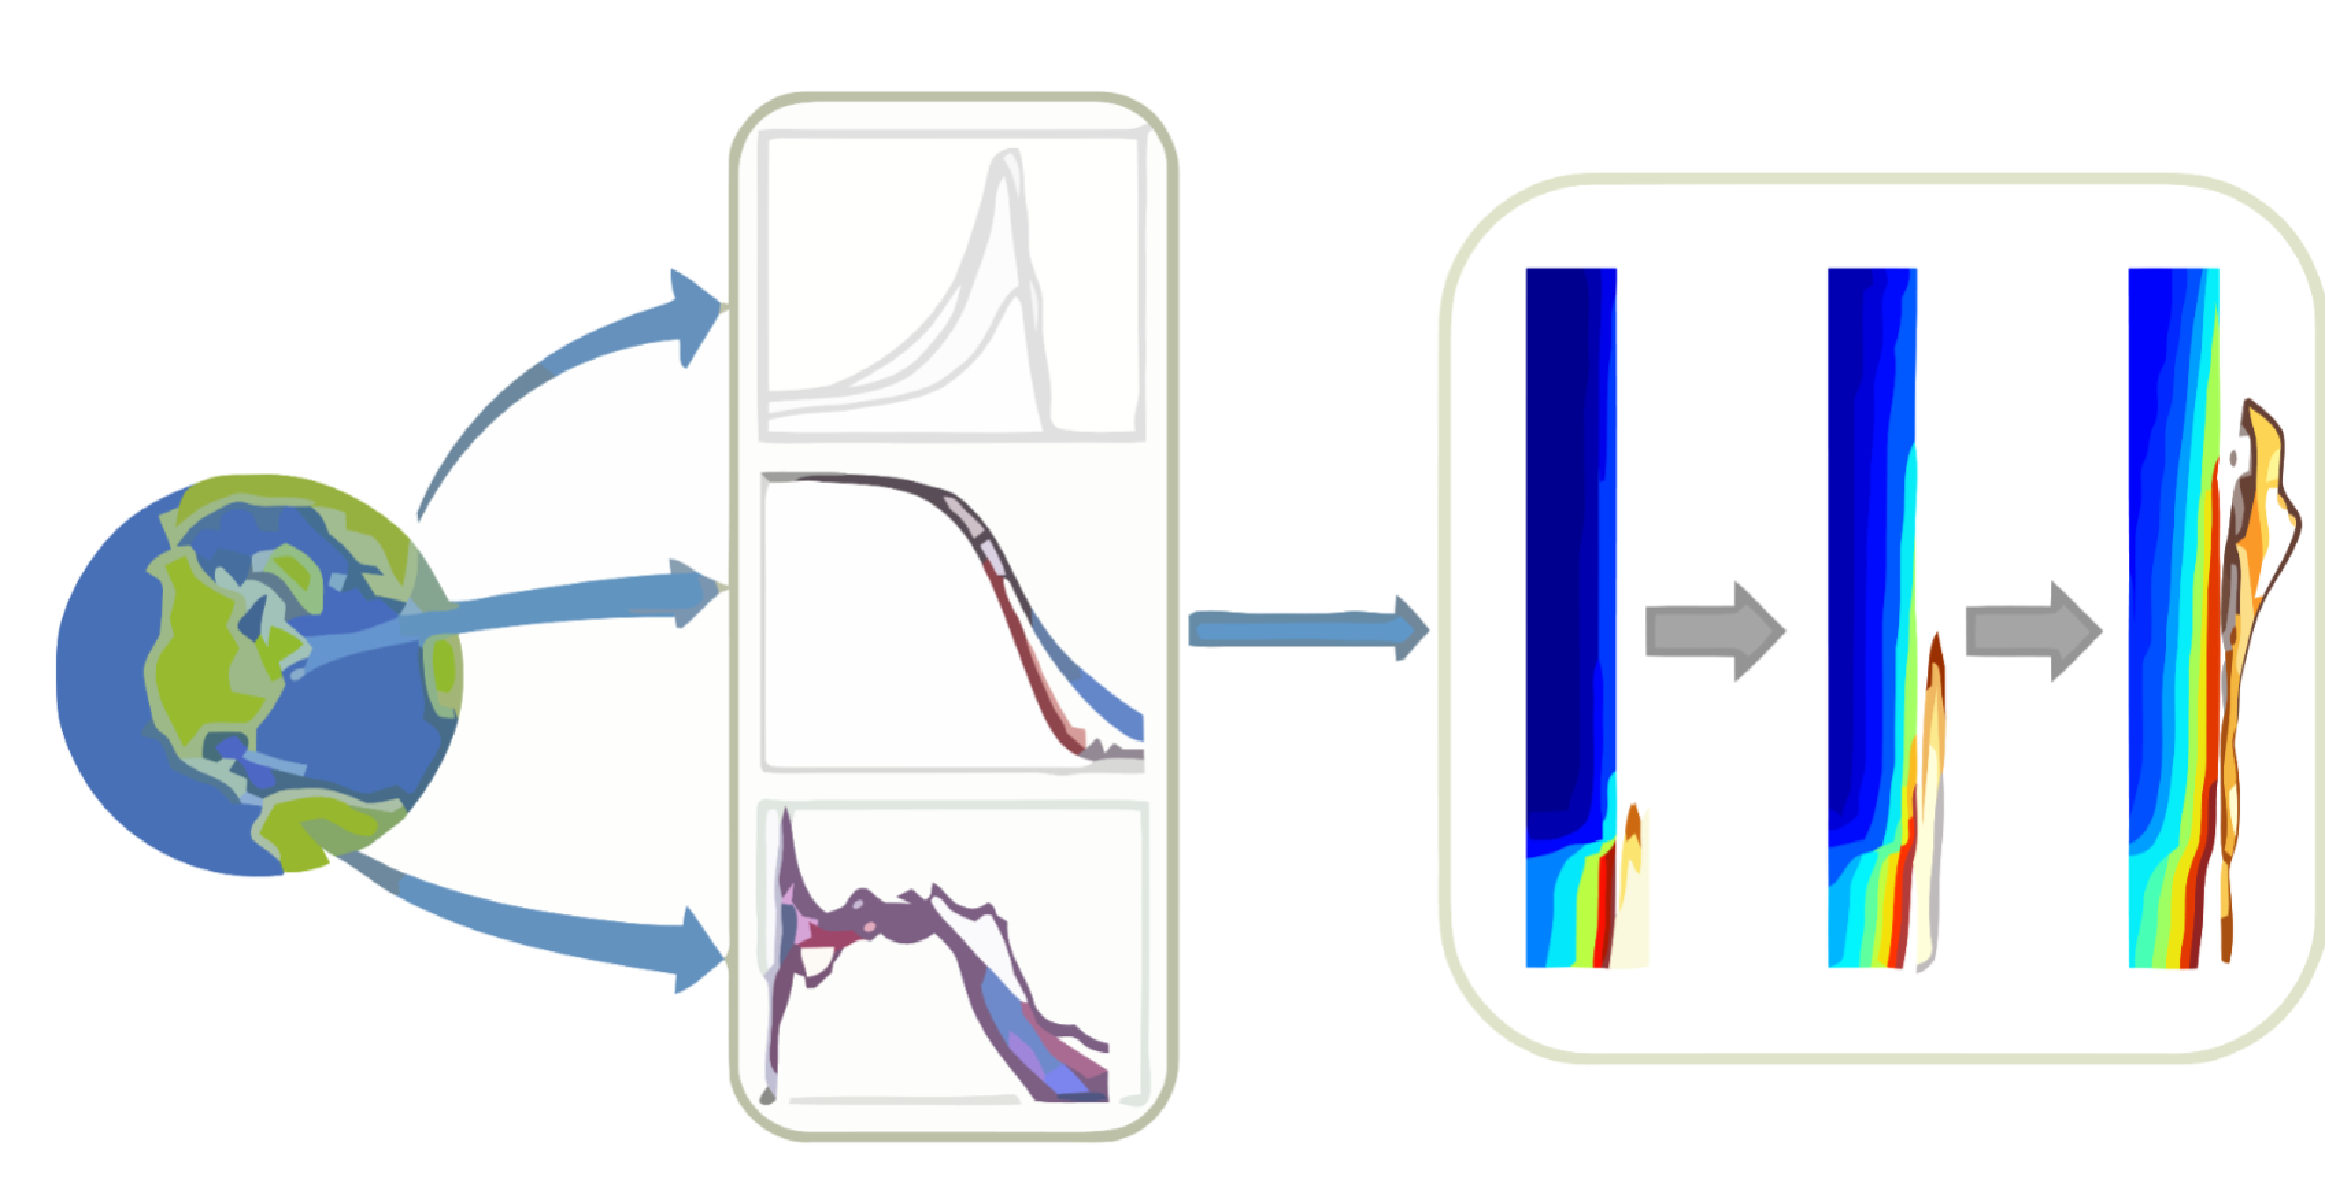
\includegraphics[width=6in]{FIGURES/MaCFP_Logo}
  \label{Cover_Image}
\end{figure}

\vfill

\begin{minipage}{0.25\textwidth}
\begin{figure}[H]

\includegraphics[width=2in]{FIGURES/IAFSSLogo}
\end{figure}
\end{minipage} \hfill
\begin{minipage}{0.7\textwidth}
\begin{flushright}
{\bf The MaCFP Condensed Phase Working Group Organizing Committee:} \\
Benjamin Batiot (University of Poitiers, France) \\
Morgan Bruns (Virginia Military Institute, USA) \\
Simo Hostikka (Aalto University, Finland) \\
Isaac Leventon (National Institute of Standards and Technology, USA) \\
Yuji Nakamura (Toyohashi University of Technology, Japan) \\
Pedro Reszka (Universidad Adolfo Ibáñez, Chile) \\
Thomas Rogaume (University of Poitiers, France) \\
Stanislav Stoliarov (University of Maryland, USA)
\end{flushright}
\end{minipage}


\newpage
\thispagestyle{empty}

\frontmatter


\chapter{Preface}

This report has been prepared on behalf of the MaCFP Condensed Phase Working Group. It is a predecisional draft copy prepared for subject matter experts to provide critical review and to ensure the integrity of the measurement data and related analysis submitted to the 2021 MaCFP Condensed Phase Workshop.

Parts of this work were prepared by the National Institute of Standards and Technology (NIST), an agency of the US government, and is not subject to copyright in the USA. Not all of the measurement data presented here has been through a formal review process. The identification of any commercial product or trade name does not imply endorsement or recommendation by NIST (or any other contributing institution). The policy of NIST is to use metric units of measurement in all its publications, and to provide statements of uncertainty for all original measurements. In this document, however, data from organizations outside NIST are shown, which may include measurements in non-metric units or measurements without uncertainty statements.

 

\newpage

\tableofcontents

\mainmatter

\pagestyle{fancy}

\chapter{Introduction}

In April 2016, it was proposed that the Measurement and Computation of Fire Phenomena (MaCFP)1 Working Group be expanded to include a subgroup dedicated to the predictive modeling of condensed phase phenomena. The MaCFP Condensed Phase Working Group was thus organized to enable the fire safety science research community to make significant progress towards establishing a common framework for the selection of experiments and the methodologies used to analyze these experiments when developing pyrolysis models. Ultimately, such a framework will support reliable computational predictions of how materials burn, how flames spread, and how fires grow in realistic fire scenarios. Key objectives of this effort include:
\begin{itemize}
 \item Cataloguing current approaches used to parameterize pyrolysis models;
 \item Developing standard data set formats for experimental data on pyrolysis;
 \item Developing requirements for data set quality and establishing a data review committee;
 \item Quantifying the inter-laboratory variability for comparable experimental datasets; and
 \item Assessing the impact of the variability of model parameters on fire growth predictions
\end{itemize}
At the first MaCFP workshop, conducted in Lund, Sweden, at the 2017 IAFSS meeting \cite{brown2018proceedings}, it was proposed that experimental data sets for pyrolysis model calibration and validation first be developed for relatively simple materials that are isotropic in nature and do not exhibit complex mechanical behavior such as melt flow, delamination or intumescence. Thus, cast black poly(methyl methacrylate), PMMA, was selected as a reference material for analysis. This material was selected because of its tendency to maintain its density while burning, insignificant melt flow, simple decomposition kinetics, and low transparency to infrared radiation. Samples of this PMMA were made available to participants and a reference document, ``Guidelines for Participation in the 2021 MaCFP Condensed Phase Workshop,'' was shared with the community to facilitate collaboration between participating institutions \cite{MaCFP_Guidelines_for_Part}.

Numerous review papers on pyrolysis model development and/or parameterization have recently been published \cite{nyazika2019pyrolysis,rogaume2019thermal, stoliarov2016parameterization,matala2012generalized}. Although multiple experimental \cite{kashiwagi1982study, hirata1985thermal, tewarson1992fire, rhodes1996burning} and computational modeling studies of the flammability response of PMMA exist in the literature \cite{consalvi2008numerical, leventon2015flame, fukumoto2018large} this effort represents the first coordinated attempt involving multiple institutions to simultaneously perform a series of pyrolysis experiments across a range of scales, characterize all relevant thermophysical properties of a fully specified material, and to compare the various methodologies for doing so.

\section{Material Selection}

The specific material of interest is a 6~mm (0.236~in) thick, black, cast PMMA manufactured by Evonik under the tradename ACRYLITE® cast black 9H01~GT. Samples were distributed to participating institutions during the summer and fall of 2019 in the form of 100~mm by 100~mm by 6~mm slabs for bench-scale experiments (e.g., cone calorimeter) and approximately 300~mg vials of powdered PMMA for micro-scale experiments (e.g., thermogravimetric analysis, TGA). Powdered samples were prepared by first pelletizing 6~mm thick slabs using an electric grinder into small (0.5~mm to 5~mm) pieces, which were then ground into a powder using a mechanical grinder with a ceramic burr.

\section{Participating Laboratories}

As of July 2020, sixteen institutions from ten different countries have submitted experimental measurements as part of the 2021 Condensed Phase MaCFP Workshop. These institutions and their countries are listed in Table~\ref{Table:Institutions} and the location of each institution is shown in Fig.~\ref{Fig:MaCFP_Map_20200831}. As this report is preliminary and further edits to experimental measurements may be required, in all figures and tables containing experimental measurements, institutions are referred to using a unique, anonymous city name. Participating labs should have received an email identifying their corresponding city names; please contact Isaac Leventon (isaac.leventon@nist.gov) if you have questions regarding this naming.

\begin{figure}[h]
  \centering
  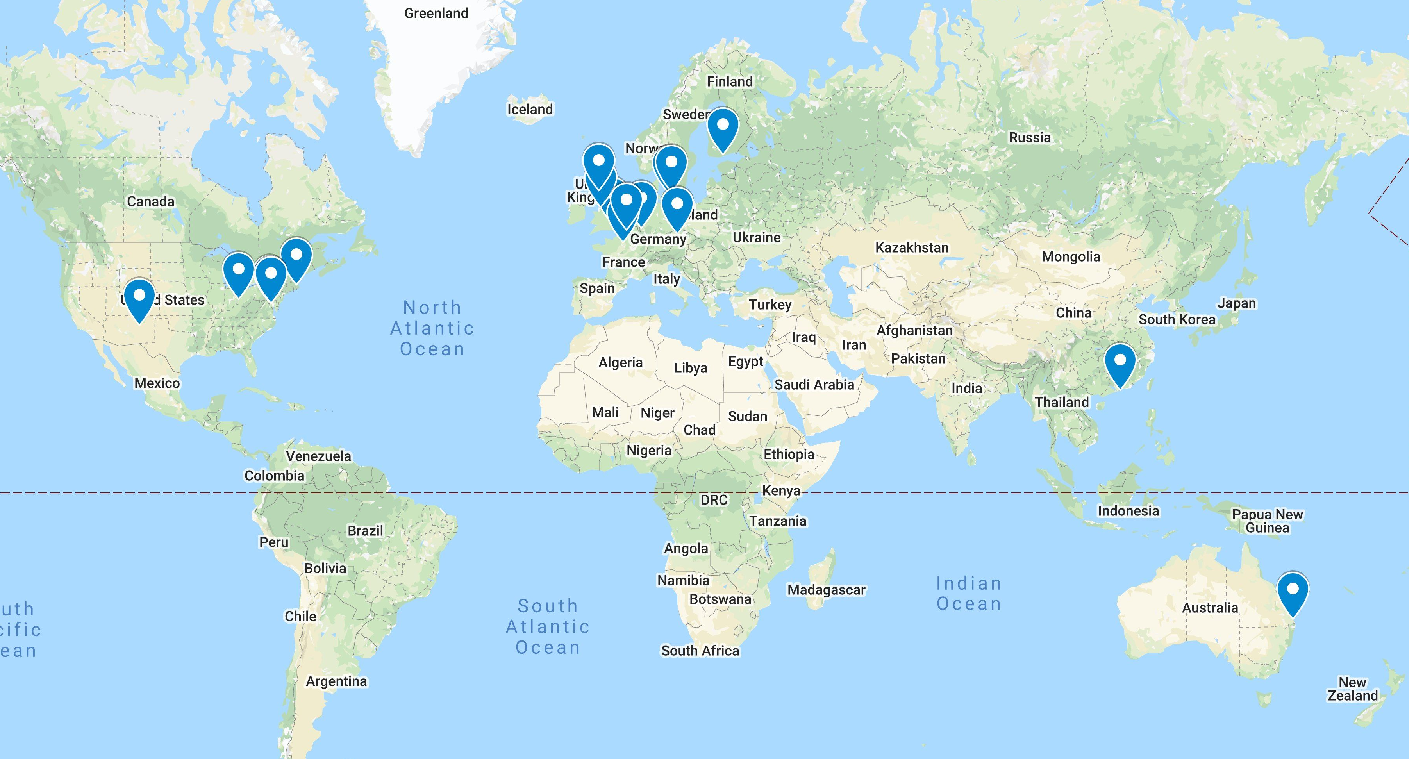
\includegraphics[width=6in]{FIGURES/MaCFP_Map}
  \caption{Locations of Institutions that provided experimental measurements for the 2021 Condensed Phase MaCFP Workshop.}
  \label{Fig:MaCFP_Map_20200831}
\end{figure}

\begin{table}
\caption{Institutions Participating in the 2021 Condensed Phase MaCFP Workshop}
\label{Table:Institutions}
\begin{center}
\begin{tabular}{|ll|}
\hline
 \textbf{Participating Institution}                                 &  \textbf{City/State, Country} \\ \hline \hline
Aalto University                                                    & Espoo, Finland \\ \hline
Dansk Brand og Sikringsteknisk Institut (DBI)                       & Copenhagen, Denmark \\ \hline
Lund University                                                     & Lund, Sweden \\ \hline
FM Global                                                           & Massachusetts, USA \\ \hline
Imperial College of London (GIDAZE+)                                & England, UK \\ \hline
Hong Kong Polytechnic University                                    & Hong Kong \\ \hline
Laboratoire Central de la Préfecture de Police (LCPP)               & Paris, France \\ \hline
National Institute of Standards and Technology (NIST)               & Maryland, USA \\ \hline
Sandia National Laboratories                                        & New Mexico, USA \\ \hline
Technical Institute of Fire Protection in Prague (TIFP)             & Prague, Czech Republic \\ \hline
University of Central Lancashire (UCLAN)                            & England, UK \\ \hline
University of Dayton Research Institute (UDRI)                      & Ohio, USA \\ \hline
University of Edinburgh                                             & Scotland, UK \\ \hline
University of Maryland (UMD)                                        & Maryland, USA \\ \hline
University of Lille - Unité Matériaux et Transformations (UMET)     & Lille, France \\ \hline
University of Queensland                                            & Queensland, Australia \\ \hline
\end{tabular}
\end{center}
\end{table}


\section{Reporting of Results: The MaCFP Repository}

Experimental measurements were submitted electronically by participating institutions and were organized and made publicly available in the MaCFP repository, which is hosted on GitHub \href{https://github.com/MaCFP/matl-db}{https://github.com/MaCFP/matl-db}. The repository was created and is managed by members of the MaCFP Organizing Committee. All measurement data submitted by each institution is organized in a single folder with the institution’s name. A consistent file naming convention is used for all test data (i.e., across all folders). File names indicate the institution name, experimental apparatus, and basic test conditions (e.g., incident heat flux or heating rate; gaseous environment). Measurement data from repeated experiments is saved in separate files, each numbered sequentially.

Also included in each folder is a README.md file that provides a description of the test conditions of all experiments conducted and submitted. Participants were asked to provide a written description of test setup and procedure and to clearly define the conditions associated with the experiments conducted, as noted in Table~\ref{Table:Tests_Performed}.

\begin{table}[ht]
\caption{Test conditions and output data requested from participants}
\label{Table:Tests_Performed}
\begin{center}
\begin{tabular}{ll}
\hline
\multicolumn{2}{c}{Test Apparatus}                                                                       \\ \hline
 \textbf{Thermogravimetric Analysis (TGA)}         &  \textbf{Differential Scanning Calorimetry (DSC)}              \\
 \textbf{Microscale Combustion Calorimetry (MCC)} &  \textbf{Cone Calorimeter}                                     \\
 \textbf{Fire Propagation Apparatus (FPA)}                  &  \textbf{Controlled Atmosphere Pyrolysis Apparatus (CAPA)}     \\
\hline
\multicolumn{2}{c}{Test Conditions}                                                                      \\ \hline
Heating Rate [K/min]                              & Radiant heat flux [kW/m$^2$]                        \\
Temperature Program:                              & Heater Temperature                                   \\
\hspace{.1in} Initial temperature                 & Extracting flow rate of the gas                      \\
\hspace{.1in} Conditioning isotherm (if used)     & Initial and Final Sample Mass                        \\
\hspace{.1in} Maximum temperature                 & Sample holder geometry and characteristics           \\
Sample mass [mg]                                  & Thermal properties of backing insulation             \\
Sample geometry (e.g., powdered)                  &                                                      \\
Calibration type, materials used, and frequency   &                                                      \\
Carrier gas and associated flow rate              &                                                      \\
Crucible type and volume                          &                                                      \\
\hline
\multicolumn{2}{c}{Test Outputs}                                                                         \\ \hline
Initial and Final Sample Mass [mg]                & Sample Surface Area [m$^2$]                             \\
Time-resolved Sample Mass [mg]                    & Initial and Final Sample Mass [mg]                   \\
Time-resolved Sample Temperature [K]              & Time-resolved Sample Mass [mg]                       \\
                                                  & Time-resolved Sample Back-Surface Temperature [K]    \\
\hline
\end{tabular}
\end{center}
\end{table}



\chapter{Experiments Conducted}

No single approach for pyrolysis model parameterization was suggested by the organizing committee of the MaCFP Condensed Phase Subgroup. In fact, a key objective of this workshop is to catalogue the current approaches used to parameterize pyrolysis models. Thus, participating institutions were encouraged to follow their own best practices when selecting and conducting experiments so that discussions could be organized at the 2021 MaCFP workshop regarding the similarities and differences of their approaches and their results (i.e., final parameterization) without explicitly requiring a final validation versus a given test.

It was expected that participating institutions would submit data from experiments such as thermogravimetric analysis (TGA), differential scanning calorimetry (DSC), the Cone Calorimeter, slab gasification experiments, and the Fire Propagation Apparatus (FPA). Although participants could conduct any experiments that they deemed necessary to provide calibration data for pyrolysis model development, a key objective of this effort was to quantify the inter-laboratory variability for comparable experimental datasets. Thus, recommended test conditions (e.g., incident heat flux in cone calorimeter tests or heating rate in TGA tests) were defined for standard experiments so that, if participants conducted any of those tests as part of their pyrolysis model development, they could do so under similar conditions, thus allowing for direct comparison of results from different laboratories.

In total, experiments were performed in eight unique apparatus under a combination of thirty-five different sets of test conditions (e.g., incident heat flux, heating rate, and/or gaseous environment). A brief description of each of the eight test apparatus used by participating institutions is provided in Sections~\ref{mg_tests} and \ref{g_tests} of this document. More information regarding these techniques is available in the literature \cite{brown2001introduction,SFPEHandbookThermalDecomp}. Detailed descriptions of the specific test conditions used by participating labs are available on the MaCFP repository \href{https://github.com/MaCFP/matl-db}{https://github.com/MaCFP/matl-db}.


\section{Milligram-Scale Tests}
\label{mg_tests}

\subsection{Thermogravimetric Analysis (TGA)}

In TGA experiments, small samples (typically 3~mg to 10~mg) are heated at a constant rate ($5\le\beta\le20$~K/min) or maintained at constant elevated temperature in a carefully controlled gaseous environment (either inert or oxidative). Time-resolved measurements of sample mass and temperature are recorded. Care should be taken to ensure that crucibles and thermocouples selected for use in TGA tests are both compatible with the sample and test conditions of interest and that the instrument is calibrated for use under those specific test conditions (i.e., atmosphere and heating rate). At the start of each day’s testing, a baseline correction should also be performed to account for artificial changes in measured sample mass due to changes in buoyancy during the heating program. Further detail regarding the principles and practices of TGA is available elsewhere \cite{coats1963thermogravimetric}.

The combination of small sample size and relatively low heating rate used in TGA experiments allows for the assumption of infinitely fast transport processes, decoupling thermal degradation reactions from heat and mass transfer effects. Analysis of TGA mass and mass loss rate data thus allows for the study of condensed-phase thermal decomposition reaction mechanisms and the determination of the kinetics of these reactions.

Twelve unique institutions submitted TGA measurements from tests conducted in four different gaseous environments at nine different heating rates. For each of these experiments, powdered samples between 2~mg and 6~mg were loaded into crucibles, weighed, and then heated (from ambient temperature through complete thermal decomposition) at a constant rate between 1~K/min and 100~K/min. Prior to heating, some samples were loaded and kept under isothermal conditions for approximately 10~min to 20~min. More information, including  apparatus specifications, calibration details, and sample preparation, conditioning, and testing procedure, is provided in the README files for each experiment. This documentation is available on the MaCFP repository \href{https://github.com/MaCFP/matl-db}{https://github.com/MaCFP/matl-db}. Tables~\ref{Table:Matrix_TGA_N2} and \ref{Table:Matrix_TGA_O2_Ar} show the number of TGA tests conducted under each combination of test conditions.

\begin{table}[ht]
\caption{Test Matrix of TGA Tests Conducted in Nitrogen; table values indicate number of tests conducted under listed test conditions}
\label{Table:Matrix_TGA_N2}
\begin{center}
\begin{tabular}{lccccccccc}
\hline
                        & \multicolumn{9}{c}{Heating Rate (K/min)}                     \\ %\hline
Institution             & 1     & 2   & 2.5 & 5   & 10    & 15  & 20  & 50  & 100      \\ \hline
Blainville-Boisbriand   &   0   & 0   & 0   & 0   & 0     & 0   & 3   & 0   & 0        \\
Chicoutimi              &   0   & 0   & 0   & 0   & 2     & 0   & 0   & 0   & 0        \\
Drummondville           &   0   & 0   & 0   & 0   & 2     & 0   & 0   & 0   & 0        \\
Gatineau                &   0   & 0   & 3   & 3   & 3     & 3   & 3   & 0   & 0        \\
Halifax                 &   0   & 0   & 0   & 0   & 1     & 0   & 0   & 0   & 0        \\
Quebec                  &   0   & 0   & 0   & 0   & 2     & 0   & 0   & 0   & 0        \\
Rimouski                &   0   & 0   & 0   & 0   & 1     & 0   & 0   & 0   & 0        \\
Rouyn-Noranda           &   0   & 0   & 0   & 0   & 3     & 0   & 0   & 0   & 0        \\
Saint John              &   0   & 0   & 0   & 0   & 1$^*$ & 0   & 0   & 0   & 0        \\
Shawinigan              &   1   & 1   & 0   & 1   & 1     & 0   & 1   & 1   & 1        \\
Sherbrooke              &   0   & 0   & 0   & 0   & 3     & 0   & 0   & 0   & 0        \\ \hline
Total                   &   1   & 1   & 3   & 4   & 19    & 3   & 7   & 1   & 1        \\ \hline
\end{tabular}
\end{center}
$^*$'Saint John' submitted a single TGA dataset, which represents average measurements from 7 repeated tests
\end{table}

\begin{table} [h]
\caption{Test Matrix of TGA Tests Conducted in Oxygen (10 or 21 vol. \% in nitrogen) or in Argon; table values indicate number of tests conducted under listed test conditions}
\label{Table:Matrix_TGA_O2_Ar}
\begin{center}
\begin{tabular}{lccccc}
\hline
              & \multicolumn{5}{c}{Heating Rate (K/min)} \\ \hline
              & 10 & 10 & 1 & 10 & 50  \\ %\hline
Institution   & $X_{\rm O_2}=0.1$ & $X_{\rm O_2}=0.21$ & \multicolumn{3}{c}{Pure Argon}  \\ \hline
Chicoutimi    & 2 & 4   & 0 & 0 & 0 \\
Drummondville & 0 & 2   & 0 & 0 & 0 \\
Halifax       & 0 & 0   & 0 & 0 & 0 \\
Moncton       & 0 & 0   & 1 & 2 & 3 \\
Quebec        & 0 & 2   & 0 & 0 & 0 \\
Sherbrooke    & 0 & 3   & 0 & 0 & 0 \\ \hline
Total         & 2 & 11  & 1 & 2 & 3 \\ \hline
\end{tabular}
\end{center}
\end{table}


\subsection{Differential Scanning Calorimetry (DSC)}

In DSC experiments, a small material sample is placed in a crucible of high thermal conductivity and heated alongside a reference crucible in a carefully controlled gaseous environment. Unlike TGA, sample mass is not measured; rather, time-resolved measurements of sample temperature and heat flow are recorded. Heat flow to the sample can be measured in two ways: (1) power compensation DSC, in which the energy (supplied by electric current) needed to maintain the sample crucible at the same temperature as the reference crucible is directly measured, or (2) heat flux DSC, in which the temperature difference between the sample and reference pans is carefully measured during heating and prior calibration of the instrument allows for the determination of heat flux as a function of this temperature difference. Further detail regarding the principles and practices of differential scanning calorimetry is available elsewhere \cite{mcnaughton2003differential}.

DSC can be used to quantify the heat capacities of materials as well as heats of reaction of endo- or exothermic condensed-phase reactions and the temperatures at which they occur. These features of interest can be determined based on the deviations of measured heat flow to the sample versus from the baseline (heat flow to empty crucibles). In DSC tests, the baseline is not necessarily easy to establish. The baseline itself may deviate from zero for a variety of reasons including a mismatch of the thermal properties of the sample and the reference material, poor positioning of crucibles themselves or of the samples within their crucible, and/or asymmetry in the construction of sample and reference holders. Excellent thermal contact between the sample, the reference pans, and the instrument and careful calibration of the instrument for the exact test conditions used in each experiment is essential to obtaining accurate measurements of sample heat capacity or heats of decomposition.

Eight institutions submitted DSC measurements from tests conducted in three different gaseous environments at five different heating rates. For most of these experiments, powdered samples between 2~mg and 6~mg were loaded into metallic crucibles, weighed, and then heated (from ambient temperature through complete thermal decomposition) at a constant rate between 5~K/min and 20~K/min. Some institutions submitted both TGA and DSC data that was obtained using a simultaneous thermal analyzer (STA). In this report, these results are presented and analyzed separately. One institution, ‘Shawinigan’, provided DSC measurements for determination of heat capacity ``by comparison with sapphire and using modulation.'' In these tests, samples were heated and cooled (three times in each test) from 190~K to 430~K. Tests were repeated using heating rates of 3~K/min, 10~K/min or 20~K/min.

More information, including  apparatus specifications, calibration details, and sample preparation, conditioning, and testing procedure, is provided in the README files for each experiment. This documentation is available in the MaCFP repository \href{https://github.com/MaCFP/matl-db}{https://github.com/MaCFP/matl-db}. Table~\ref{Table:Matrix_DSC} shows the number of DSC tests conducted by each institution under each combination of test conditions.

\begin{table}[ht]
\caption{Test Matrix of DSC Tests Conducted in Pure Nitrogen; table values indicate number of tests conducted under listed test conditions}
\label{Table:Matrix_DSC}
\begin{center}
\begin{tabular}{lcccccccc}
							\hline
                      & \multicolumn{8}{c}{Heating Rate (K/min)} \\ 
                      & 3 & 10 & 20 & 10 & 10 & 1  & 10 & 50 \\ 
                      \hline
Institution           & \multicolumn{3}{c}{Pure Nitrogen} & $X_{\rm O_2}=0.1$ & $X_{\rm O_2}=0.21$ & \multicolumn{3}{c}{Pure Argon}  \\ \hline
Blainville-Boisbriand & 0 & 0     &     3 & 0 & 0 & 0 & 0 & 0 \\
Chicoutimi            & 0 & 2     &     0 & 2 & 4 & 0 & 0 & 0 \\
Drummondville         & 0 & 2     &     0 & 0 & 2 & 0 & 0 & 0 \\
Moncton               & 0 & 0     &     0 & 0 & 0 & 1 & 2 & 3 \\
Quebec                & 0 & 2     &     0 & 0 & 2 & 0 & 0 & 0 \\
Rimouski              & 0 & 1     &     0 & 0 & 0 & 0 & 0 & 0 \\
Saint John            & 0 & 1$^*$ &     0 & 0 & 0 & 0 & 0 & 0 \\
Shawinigan            & 1 & 2     &     2 & 0 & 0 & 0 & 0 & 0 \\ \hline
Total                 & 1 & 10    &     5 & 2 & 8 & 1 & 2 & 3 \\ \hline
\end{tabular}
\end{center}
$^*$Saint John submitted a single DSC dataset, which represents average measurements from 7 repeated tests
\end{table}

\subsection{Microscale Combustion Calorimetry (MCC)}

In MCC experiments, mg-scale samples are heated in a carefully controlled (typically anaerobic) gaseous environment, similar to TGA. Gaseous pyrolyzates produced by the sample are transported in an inert gas stream to a high-temperature furnace where they are mixed with excess oxygen and allowed to burn to completion. Measurement of total gas flow and oxygen concentration downstream of the furnace allows for the calculation of sample heat release rate due to this non-flaming combustion, based on the principle of oxygen consumption calorimetry. The heat of complete combustion is obtained from the time integral of this heat release rate and measurements of initial and final sample mass. Further detail regarding the principles and practices of MCC is available elsewhere \cite{lyon2013principles}.

Two institutions provided measurement data from repeated MCC tests conducted in a pure nitrogen environment. In each test, powdered samples between 4~mg and 7~mg were loaded into ceramic crucibles, weighed, and then introduced into the MCC pyrolyzer for 10~min at 348.15~K. Samples were then heated from this  temperature through complete thermal decomposition at a constant heating rate of 60~K/min. Additional information, including  apparatus specifications, calibration details, and sample preparation, conditioning, and testing procedure, is provided in the README files for each experiment, which can be found in the MaCFP repository \href{https://github.com/MaCFP/matl-db}{https://github.com/MaCFP/matl-db}.

\section{Gram-Scale Tests}
\label{g_tests}

\subsection{Cone Calorimeter}

In cone calorimetry experiments, gram-scale samples (typically 10~cm square, 6~mm thick) are placed on a layer of thermal insulation inside of a steel holder and exposed to a conical, radiant heater capable of providing an external heat flux of 10~kW/m$^2$ to 75~kW/m$^2$. Samples can be supported in either the horizontal or vertical configuration (typically horizontal) with or without a spark igniter. This provides (nominally) a one-dimensional heating scenario where sample slabs can burn freely in well-ventilated, open-atmosphere conditions. Samples are supported above a load cell and positioned beneath a well-instrumented exhaust hood, capable of providing oxygen consumption measurements. Thus, the apparatus produces time-resolved measurements of sample mass loss and heat release rates. Further detail regarding the operating principles, best practices, complete capabilities, and analysis techniques of cone calorimetry is available elsewhere \cite{babrauskas1984development, SFPEHandbookCone, astm1354standard}.

Eleven institutions submitted experimental measurements from 59 unique cone calorimeter tests conducted using an applied external heat flux of 25, 50, or 65~kW/m$^2$. For most of these tests, samples were 6~mm thick and 10~cm square. 'Blainville-Boisbriand' repeated experiments using smaller, circular samples, which has been reported to improve repeatability of experiments \cite{vermina2019experimental}. Tests were conducted both with and without frames (to keep samples in place within their holders) using a variety of backing insulation layers. Both of these features may impact the burning behavior of samples during experiments. Additional information, including apparatus specifications and calibration details, backing insulation thermal conductivity, and sample preparation, conditioning, and testing procedure, is provided in the README files for each experiment, which can be found in the MaCFP repository \href{https://github.com/MaCFP/matl-db}{https://github.com/MaCFP/matl-db}. Table~\ref{Table_6} lists the number of cone calorimeter experiments conducted under each combination of test conditions.

\begin{table}[ht]
\caption{Test Matrix of Cone Calorimeter Experiments; table values indicate number of tests conducted under listed test conditions}
\label{Table_6}
\begin{center}
\begin{tabular}{lccc}
\hline
                        & \multicolumn{3}{c}{Incident Heat Flux (kW/m$^2$)} \\ %\hline
Institution             & 25 & 50 & 65       \\ \hline
Baie-Comeau             & 0     & 0     & 3  \\
Blainville-Boisbriand   & 6     & 3     & 3  \\
Cape-Breton             & 3     & 0     & 3  \\
Chicoutimi              & 2     & 0     & 2  \\
Drummondville           & 2     & 0     & 2  \\
Gatineau                & 4     & 0     & 4  \\
Halifax                 & 3     & 0     & 0  \\
Quebec                  & 3     & 0     & 3  \\
Rimouski                & 1     & 0     & 1  \\
Rouyn-Noranda           & 3     & 0     & 4  \\
Sherbrooke              & 2     & 0     & 2  \\ \hline
Total                   & 29    & 3     & 27 \\ \hline
\end{tabular}
\end{center}
\end{table}

\subsection{Anaerobic Gasification}

Six institutions conducted a total of 27 anaerobic gasification experiments using three different experimental apparatus: a Controlled Atmosphere Cone Calorimeter, a Fire Propagation Apparatus (FPA), or a Controlled Atmosphere Pyrolysis Apparatus (CAPA). All three apparatus produce nominally one-dimensional heating of gram-scale samples (here, 6~mm thick) in an anaerobic environment. Table~\ref{Table_7} lists the number of gasification experiments conducted under each combination of apparatus type and test conditions.

\begin{table}[ht]
\caption{Test Matrix of Gasification Experiments; table values indicate number of tests conducted under listed test conditions}
\label{Table_7}
\begin{center}
\begin{tabular}{lcccccccc}
\hline
                         & \multicolumn{3}{c}{Controlled Atmosphere Cone} & \multicolumn{2}{c}{CAPA} & \multicolumn{3}{c}{FPA}     \\ \hline
                         & \multicolumn{8}{c}{Incident Heat Flux (kW/m$^2$)}                                                       \\ %\hline
Institution              & 25 & 50 & 65 & 25 & 60 & 25 & 50 & 65                                                                   \\ \hline
Baie-Comeau              & 0  & 0  & 3  & 0  & 0  & 0  & 0  & 0                                                                    \\
Blainville-Boisbriand    & 3  & 2  & 0  & 0  & 0  & 0  & 0  & 0                                                                    \\
Charlottetown            & 0  & 0  & 0  & 0  & 0  & 3  & 3  & 3                                                                    \\
Chicoutimi               & 0  & 0  & 0  & 0  & 0  & 2  & 0  & 2                                                                    \\
Quebec                   & 0  & 0  & 2  & 0  & 0  & 0  & 0  & 0                                                                    \\
Saint John               & 0  & 0  & 0  & 2  & 2  & 0  & 0  & 0                                                                    \\ \hline
Total                    & 3  & 2  & 5  & 2  & 2  & 5  & 3  & 5                                                                    \\ \hline
\end{tabular}
\end{center}
\end{table}


\paragraph{Controlled Atmosphere Cone Calorimetry}

In controlled atmosphere cone calorimetry, a standard cone calorimeter (described above) is modified by building an enclosure around the heater and the sample platform. By supplying a well-defined mixture of nitrogen, oxygen, and/or air to this enclosure, a reduced oxygen environment can be maintained around the sample. Further information regarding the development of controlled atmosphere cone calorimetry and an explanation of how the controlled‐atmospheres unit is operated is provided elsewhere \cite{babrauskas1992cone}.

\paragraph{Controlled Atmosphere Pyrolysis Apparatus (CAPA)}

The most recent version of this apparatus, CAPA~II, was used to obtain the reported data. CAPA~II provides a well-defined, axi-symmetric, one-dimensional heating environment in which a disc-shaped sample (7~cm diameter) is exposed to radiant heat supplied by the heating element of a cone calorimeter. The oxygen concentration around the sample can be reduced below 1~\% by supplying a co-flow of pure nitrogen around the sample. The sample rests on a painted copper foil exposed to the atmosphere to enable a non-intrusive back surface temperature measurement. In each experiment, time-resolved measurements of sample mass, back surface temperature, and sample profile evolution are recorded simultaneously. Additional information about CAPA~II, including quantification of boundary conditions, measurement capabilities and technique, and sample preparation, conditioning, and testing procedure, is available elsewhere \cite{swann2017controlled}.

\paragraph{Fire Propagation Apparatus (FPA)}

In the FPA, for ignition, pyrolysis, and combustion tests (i.e., not for flame spread), horizontal samples (either 10~cm square or in diameter) are supported on a mass balance and exposed to external radiant heat from four quartz heaters typically operating at significantly higher temperatures than the heating element of the cone calorimeter. Samples are surrounded by a 17~cm diameter quartz tube, which allows for the co-flow of well-regulated mixtures of nitrogen and/or oxygen around the sample, thus allowing for the generation of an anerobic environment. Additional information about the FPA, including further discussion on its measurement capabilities, and sample preparation, conditioning, and testing procedure, is available elsewhere \cite{astm2058standard}.

\subsection{Thermal Conductivity and Diffusivity}

``Direct measurements'' of thermal conductivity and diffusivity were provided by one institution, using two separate apparatus: TPS hot disk \cite{gustafsson1991transient} and Laser Flash \cite{NeztschLFA}. The reader is referred to the technical reference guide and/or user’s manuals of each of these instruments for further information regarding their operating principles and related test procedures.



\chapter{Experimental Results}

In this section, experimental measurements from both mg- and g-scale tests are presented. When tests were conducted under the same nominal experimental conditions (e.g., heating rate, incident heat flux, and/or gaseous environment) and when data provided by different institutions showed qualitative agreement, average curves (e.g., heat release or mass loss rate vs. time or temperature) and related uncertainties are calculated. Specifically, type A uncertainties~\cite{taylor1994nist} are reported for all data as two standard deviations of the mean calculated over at least three independent observations, unless otherwise stated.

It should be noted that some variations between datasets are simply stochastic (i.e., random, unavoidable noise in repeated tests); however, others may result from systematic causes such as calibration differences in mg-scale experiments or sample holder and/or insulation type in g-scale experiments. Consequently, although clear outliers are not considered when calculating average curves (see further discussion throughout this section on how outliers are identified), care should be taken to understand if/how underlying differences in test conditions or procedure may have impacted the response of samples during experiments and thus how this may affect the final averaged dataset. Ultimately, average curves represent the aggregate of data as received, some of which may require corrections by the original submitting institution (e.g., if a dataset was incorrectly labeled or submitted).

The measurement data presented here is provided with limited processing and should be considered as a preliminary summary to highlight the information that is available in the MaCFP repository \href{https://github.com/MaCFP/matl-db}{https://github.com/MaCFP/matl-db} as of August 26, 2020. Further analysis of these results, including determination if correlation or causation of similarities or differences in datasets submitted by different institutions can be found (e.g., due to variations in instrument design, calibration or test procedure, and/or sample holder), will be provided in a future report.

\section{Milligram-Scale Tests}

\subsection{Thermogravimetric Analysis (TGA)}
\label{TGA_analysis}

\subsubsection{Heating Rate}

All TGA experiments submitted to this workshop were performed at constant heating rates between 1~K/min and 100~K/min. In practice, actual heating rate may vary throughout the course of experiments (especially at their start, while the TGA furnace is heating up). Figures~\ref{Fig:dTdt_TGA_10K} and \ref{Fig:dTdt_TGA_20K} show actual time-resolved heating rates in tests conducted, nominally, at $\beta$ = 10 and 20 K/min, respectively. In either figure, each curve represents the mean instantaneous heating rate as calculated from repeated experiments conducted by the same institution, under the same gaseous environment and target heating rate. When multiple curves are shown for the same institution on Fig.~\ref{Fig:dTdt_TGA_10K}, they represent average heating rates measured in tests conducted under different gaseous environments (e.g., pure nitrogen, pure argon, or 10 vol.~\% to 21 vol.~\% oxygen in nitrogen).

As shown here, the actual heating rate can vary significantly during the early stages of testing (i.e., as samples are first heated from 50~K to 150~K above their initial temperature) before the heating rate, $\beta$, finally reaches its target value. For experiments conducted by a single institution at the same nominal heating rate but under different gaseous environments, no systematic differences in time-resolved heating rates were observed.

\begin{figure}
  \centering
  \includegraphics[width=5.5in]{SCRIPT_FIGURES/dTdt_TGA_10K}
  \caption{Average (of repeated experiments conducted by a single institution in the same gaseous environment) instantaneous heating rate during TGA experiments conducted at a nominal heating rate of $\beta=10$ K/min. Repeated curves for the same institution represent measurement data from tests conducted in different gaseous environments. Note: TGA tests submitted by ‘Gatineau’ at 10~K/min appear to have been conducted at 20~K/min.}
  \label{Fig:dTdt_TGA_10K}
\end{figure}

\begin{figure}
  \centering
  \includegraphics[width=5.5in]{SCRIPT_FIGURES/dTdt_TGA_20K}
  \caption{Average (of repeated experiments conducted by a single institution) reported instantaneous heating rate during TGA experiments conducted at a nominal heating rate of $\beta=20$ K/min; all tests conducted in pure nitrogen.}
  \label{Fig:dTdt_TGA_20K}
\end{figure}


\subsubsection{Mass Fraction and Mass Loss Rate}

The key measurements recorded during TGA tests are sample mass, $m$~(mg), and temperature, $T$~(K) (and the time, $t$~(s), at which these two values are recorded).  Both $m$ and $T$ were reported as time-resolved measurements. Prior to further analysis, sample mass was normalized by initial mass, $m_0$, which was calculated as the average value recorded during the first 5~s of the experiment.

Tests were run at constant heating rates and both sample mass and temperature were reported at regular time or temperature intervals; effectively this meant that sample mass was reported, in most experiments, every 0.5~K (the full range of reporting frequencies in datasets submitted by different institutions varied between 0.1~K and 1~K per mass measurement, with two institutions submitting data with 5~K or 6.7~K resolutions). Reporting frequency was not necessarily constant and, due to the nature of the experiment, measured sample temperature could actually decrease from one time step to the next.

For all tests, normalized mass, $m/m_0$, and time, $t$, signals were thus first processed using linear interpolation such that they were each reported at the same regular intervals (i.e., every 0.5~K). For two experimental datasets, ‘Chicoutimi’ and ‘Rimouski', the original reporting frequency of one or more of these signals was deemed too coarse (every 5~K or 6.7~K) for this linear interpolation, thus this processing was not applied.
Prior to further analysis, noise in all individual $m/m_0$ curves was reduced by applying a Savitzky-Golay filter (third order polynomial fit; 31 data point range). These fitting parameters were determined by trial and error, and future work will examine optimizing the choice of these parameters. Figure~\ref{Fig:TGA_N2_10K_1} shows the effect of this filter on a representative TGA dataset (data submitted by ‘Halifax’ from a test in pure nitrogen at 10~K/min).

Normalized mass loss rate was then calculated for each replicate $j$ at each temperature, $T_i$, as the numerical derivative of filtered sample mass curves across a 1~K interval, as follows: 
\begin{equation}
   \frac{\dot{m}_{i,j}}{m_{0,j}} = \frac{1}{m_{0,j}}\frac{\left(m_{i-1,j}-m_{i+1,j}\right)}{\left(t_{i+1}-t_{i-1}\right)}
\end{equation}
In this way, the time step, $\Delta t$, needed for this calculation could vary (see previous discussion on heating rates) but it would always correspond to the time needed for sample mass to increase by 1~K).

Figure~\ref{Fig:TGA_N2_10K_1} shows the effect of applying this Savitzky-Golay filter to a particularly noisy set of TGA measurements. Here, filtered and unfiltered mass data is plotted (left axis; green and blue curves, respectively) along with filtered and unfiltered mass loss rate data (right axis; black and red curves, respectively). With this filter, random noise in the signal is cleanly removed but meaningful signal data remains; relevant mass loss events are not over-smoothed; no shift is observed in the onset or peak temperature of reactions, which could occur if a larger time interval, $\Delta t$, were used to smooth calculated mass loss rate; and the peak mass loss rate is well captured. Given the effectiveness that this filter has demonstrated, it has been applied to all TGA measurements submitted to this workshop, prior to further analysis.

\begin{figure}[h!]
  \centering
  \includegraphics[width=5in]{SCRIPT_FIGURES/TGA_N2_10K_1}
  \caption{Filtered and unfiltered mass data from a single TGA experiment conducted by ‘Halifax’ in pure nitrogen at 10~K/min as well as the resulting mass loss rate curves calculated from this mass data.}
  \label{Fig:TGA_N2_10K_1}
\end{figure}

Figures~\ref{Fig:TGA_N2_5K} through \ref{Fig:TGA_N2_20K} show measurement data from 4, 19, and 7 repeated tests conducted in pure nitrogen at nominal heating rates of $\beta$ = 5, 10 and 20~K/min, respectively. Figure~\ref{Fig:TGA_N2_10K} also includes TGA measurements from ‘Moncton’, which conducted two anaerobic tests at 10~K/min in pure argon. Figure~\ref{Fig:TGA_O2-21_10K} shows measurements from 11 repeated tests conducted in oxygen and nitrogen ($X_{\rm O_2}=0.21$) at a nominal heating rate of $\beta=10$~K/min.

Based on these measurements, average TGA curves and an estimate of measurement uncertainty were calculated for each of these conditions. An effort was made to include as much data as possible in the generation of these average curves; however, clear outliers (full curves, not just individual data points) were not used for the calculation of mean and standard deviation values. These datasets are still plotted in Figs.~\ref{Fig:TGA_N2_5K} through \ref{Fig:TGA_O2-21_10K} with a note identifying them as outliers in the captions below their respective figures. For TGA measurements, datasets were defined as outliers, for example, when additional mass loss events were observed (‘Quebec’ tests in N$_2$ at 10~K/min), peak mass loss rates were greater than $50$~\% of the average of all other data, or a temperature shift of approximately 20~K or greater was observed in measurement results.

For brevity, this document supplies figures of TGA measurement data only when repeated measurements under those test conditions were supplied by multiple labs. Normalized mass and mass loss rate curves (individual test data, along with average curves) from all TGA experiments conducted by all labs and under all experimental conditions (all heating rates and gaseous environments) are supplied in the Supplemental Information document.

\begin{figure} [p]
\centering
\begin{subfigure}[b]{0.85\textwidth}
   \includegraphics[width=1\linewidth]{SCRIPT_FIGURES/TGA_N2_5KMass}
   \caption{}
   \label{Fig:TGA_N2_5KMass}
\end{subfigure}

\begin{subfigure}[b]{0.85\textwidth}
   \includegraphics[width=1\linewidth]{SCRIPT_FIGURES/TGA_N2_5Kdmdt}
   \caption{}
   \label{Fig:TGA_N2_5Kdmdt}
\end{subfigure}

  \caption{Normalized (a) mass and (b) mass loss rate of TGA tests conducted in pure nitrogen at a nominal heating rate of $\beta=5$~K/min.}
  \label{Fig:TGA_N2_5K}
\end{figure}

\begin{figure} [p]
\centering
\begin{subfigure}[b]{0.85\textwidth}
   \includegraphics[width=1\linewidth]{SCRIPT_FIGURES/TGA_N2_10KMass}
   \caption{}
   \label{Fig:TGA_N2_10KMass}
\end{subfigure}

\begin{subfigure}[b]{0.85\textwidth}
   \includegraphics[width=1\linewidth]{SCRIPT_FIGURES/TGA_N2_10Kdmdt}
   \caption{}
   \label{Fig:TGA_N2_10Kdmdt}
\end{subfigure}

  \caption{Normalized (a) mass and (b) mass loss rate of TGA tests conducted in pure nitrogen (or pure argon, ‘Moncton’) at a nominal heating rate of $\beta = 10$ K/min. The following datasets are identified as outliers and will not be used for the calculation of mean and standard deviation values: Gatineau (clearly too high, likely conducted at 20~K/min; see Fig. 2); Quebec (two peaks); Rouyn-Noranda (~20~K shift in temperature).}
  \label{Fig:TGA_N2_10K}
\end{figure}

\begin{figure}[p]
\centering
\begin{subfigure}[b]{0.85\textwidth}
   \includegraphics[width=1\linewidth]{SCRIPT_FIGURES/TGA_N2_20KMass}
   \caption{}
   \label{Fig:TGA_N2_20KMass}
\end{subfigure}

\begin{subfigure}[b]{0.85\textwidth}
   \includegraphics[width=1\linewidth]{SCRIPT_FIGURES/TGA_N2_20Kdmdt}
   \caption{}
   \label{Fig:TGA_N2_20Kdmdt}
\end{subfigure}

  \caption{Normalized (a) mass and (b)mass loss rate of TGA tests conducted in pure nitrogen at a nominal heating rate of $\beta=20$~K/min.}
  \label{Fig:TGA_N2_20K}
\end{figure}


\begin{figure}
\centering
\begin{subfigure}[b]{0.85\textwidth}
   \includegraphics[width=1\linewidth]{SCRIPT_FIGURES/TGA_O2-21_10KMass}
   \caption{}
   \label{Fig:TGA_O2-21_10KMass}
\end{subfigure}

\begin{subfigure}[b]{0.85\textwidth}
   \includegraphics[width=1\linewidth]{SCRIPT_FIGURES/TGA_O2-21_10Kdmdt}
   \caption{}
   \label{Fig:TGA_O2-21_10Kdmdt}
\end{subfigure}

  \caption{Normalized (a) mass and (b) mass loss rate of TGA tests conducted in oxygen and nitrogen ($X_{\rm O_2}=0.21$) at a nominal heating rate of $\beta=10$~K/min.}
  \label{Fig:TGA_O2-21_10K}
\end{figure}

When repeated measurements were available (submitted by the same or different lab(s) and conducted under the same incident heating conditions and gaseous environment) average mass loss rate was calculated at each temperature, $T_i$, as the average value reported from all repeated tests, $j$:
\begin{equation}
\overline{\left(\frac{\dot{m}}{m_0}\right)_i} = \frac{1}{\sum_{j=1}^{N_j}N_i} \sum_{j=1}^{N_j} \sum_{i'=i-n}^{i+n} \frac{\dot{m}_{i',j}}{m_{0,j}}
\end{equation}
where $N_i$ is equal to the number of measurements from an individual experiment, $j$, reported in the interval $(i-n) \leq i \leq (i+n)$ and $n$ is chosen based on whether the data is from the same laboratory or not. $N_j$ is the number of replicate tests. The standard deviation of the mean was calculated:
\begin{equation}
  \sigma_i^2 = \frac{1}{(\sum_{j=1}^{N_j}N_i)((\sum_{j=1}^{N_j}N_i)-1)} \sum_{j=1}^{N_j} \sum_{i'=i-n}^{i+n}  \left( \frac{\dot{m}_{i',j}}{m_{0,j}} - \overline{\left(\frac{\dot{m}}{m_0}\right)_i} \right)^2
\end{equation}
When the average and standard deviation of the mean were calculated using data provided by the same lab (except for ‘Chicoutimi’ and ‘Rimouski’), $n=2$ because it is assumed that variations in these repeated measurements should be minimal within a 4~K interval when tests are conducted by the same institution (these values are plotted in the Supplemental Information document). When the average and standard deviation of the mean were calculated across all labs (or for ‘Chicoutimi’ and ‘Rimouski’, due to coarser data reporting frequency), $n=0$ because greater variability is expected between these individual tests (or data was simply not reported at a high enough frequency to allow for such calculations).

Figure~\ref{Fig:TGA-N2_5_10_20K} plots average mass and mass loss rate curves from anaerobic TGA tests conducted at 5, 10, and 20~K/min on a single set of axes. Figure~\ref{Fig:TGA_O2-21_10K_w_avg} plots average mass and mass loss rate curves along with measurements from 11 individual tests conducted in oxygen and nitrogen ($X_{\rm O_2}=0.21$) at a nominal heating rate of $\beta=10$~K/min; this allows for a qualitative representation of the ‘fit’ of this average curve to repeated measurements submitted by various institutions. In each plot (Figs.~\ref{Fig:TGA-N2_5_10_20K} and ~\ref{Fig:TGA_O2-21_10K_w_avg}) average mass and mass loss rate is plotted as a solid curve surrounded by a shaded area, which represents two standard deviations of the mean, $2 \sigma_i$.

\begin{figure}[p]
\centering
\begin{subfigure}[b]{0.9\textwidth}
   \includegraphics[width=1\linewidth]{SCRIPT_FIGURES/TGA-N2_5_10_20K_Mass}
   \caption{}
   \label{Fig:TGA-N2_5_10_20K_Mass}
\end{subfigure}

\begin{subfigure}[b]{0.9\textwidth}
   \includegraphics[width=1\linewidth]{SCRIPT_FIGURES/TGA-N2_5_10_20K_dmdt}
   \caption{}
   \label{Fig:TGA-N2_5_10_20K_dmdt}
\end{subfigure}

  \caption{Average normalized (a) mass and (b) mass loss rate of TGA tests conducted in pure nitrogen at $\beta$ = 5, 10, and 20~K/min. Average curves are calculated using all submitted data from tests conducted under the same conditions, excluding outliers, as noted above; shaded areas represent $2\sigma_i$. Note: the average measurements plotted at 10~K/min include data from two anaerobic tests conducted at 10~K/min in pure argon.}
  \label{Fig:TGA-N2_5_10_20K}
\end{figure}


\begin{figure}[p]
\centering
\begin{subfigure}[b]{0.9\textwidth}
   \includegraphics[width=1\linewidth]{SCRIPT_FIGURES/TGA_O2-21_10KMass_w_avg}
   \caption{}
   \label{Fig:TGA_O2-21_10KMass_w_avg}
\end{subfigure}

\begin{subfigure}[b]{0.9\textwidth}
   \includegraphics[width=1\linewidth]{SCRIPT_FIGURES/TGA_O2-21_10Kdmdt_w_avg}
   \caption{}
   \label{Fig:TGA_O2-21_10Kdmdt_w_avg}
\end{subfigure}

  \caption{Normalized (a) mass and (b) mass loss rate of TGA tests conducted in oxygen and nitrogen ($X_{\rm O_2}=0.21$) at a nominal heating rate of $\beta=10$~K/min; shaded grey areas represent $2\sigma_i$.}
  \label{Fig:TGA_O2-21_10K_w_avg}
\end{figure}

\newpage
\subsubsection{Tabulated values of interest}

The peak normalized mass loss rate and the temperature at which it was recorded was calculated for each TGA experiment. Additionally, an ``onset'' temperature, defined as the temperature at which the normalized mass loss rate exceeds 10~\% of its peak value, was calculated. The mean and standard deviation of each of these values are reported in Tables~\ref{Table_8}, \ref{Table_9}, and \ref{Table_10}, respectively, for TGA experiments conducted under the most commonly performed test conditions submitted by all institutions. Here, the reported uncertainty is one standard deviation of the average value of measurements made by one organization at one exposure level.

\begin{table}[h!]
\caption{Peak normalized mass loss rate (s$^{-1}$) in TGA Experiments}
\label{Table_8}
\begin{center}
\begin{tabular}{|l|cc|cc|cc|cc|}
\hline
                        & \multicolumn{6}{|c|}{Pure Nitrogen$^D$} & \multicolumn{2}{|c|}{$X_{\rm O_2}=0.21$}                                                       \\  \hline
                        & \multicolumn{2}{|c|}{5 K/min} & \multicolumn{2}{|c|}{10 K/min}    & \multicolumn{2}{|c|}{20 K/min} & \multicolumn{2}{|c|}{10 K/min}      \\  \hline
Institution             & Mean        & Std Dev         & Mean           & Std Dev          & Mean       & Std Dev           & Mean        & Std Dev               \\  \hline
Blainville-Boisbriand   & -           & -               & -              & -                & 5.3E-03    & 1.6E-04           & -           & -                     \\
Chicoutimi              & -           & -               & 2.8E-03$^A$    & 3.5E-05$^A$      & -          & -                 & 3.2E-03     & 8.4E-04               \\
Drummondville           & -           & -               & 2.9E-03        & 1.2E-04          & -          & -                 & 3.2E-03$^A$ & 9.5E-05$^A$           \\
Gatineau                & 1.3E-03     & 2.3E-05         & 5.2E-03        & 1.2E-04          & 5.2E-03    & 1.2E-04           & -           & -                     \\
Halifax                 & -           & -               & 3.3E-03        & B                & -          & -                 & -           & -                     \\
Moncton                 & -           & -               & 3.1E-03$^{AD}$ & 6.6E-05$^{AD}$   & -          & -                 & -           & -                     \\
Quebec                  & -           & -               & 1.8E-03$^C$    & 1.0E-05$^C$      & -          & -                 & 3.3E-03$^A$ & 2.5E-04$^A$           \\
Rimouski                & -           & -               & 2.8E-03        & B                & -          & -                 & -           & -                     \\
Rouyn-Noranda           & -           & -               & 2.7E-03        & 3.2E-05          & -          & -                 & -           & -                     \\
Saint John              & -           & -               & 3.0E-03        & B                & -          & -                 & -           & -                     \\
Shawinigan              & 1.6E-03     & B               & 3.1E-03        & B                & 6.2E-03    & B                 & -           & -                     \\
Sherbrooke              & -           & -               & 2.8E-03        & 3.0E-05          & -          & -                 & 3.8E-03     & 7.7E-05               \\  \hline
\end{tabular}
\end{center}
$^A$Calculated based on two values \\
$^B$Standard deviation not calculated, only one experimental dataset provided \\
$^C$Suspected error in submitted dataset, see mass loss rate in Fig. \ref{Fig:TGA_O2-21_10K}\\
$^D$Moncton experiments were conducted in Argon
\end{table}


\begin{table}[p]
\caption{Temperature, $T_{\rm max}$ (K), at which the peak mass loss rate is observed in TGA Experiments}
\label{Table_9}
\begin{center}
\begin{tabular}{|l|cc|cc|cc|cc|}
\hline
                        & \multicolumn{6}{|c|}{Pure Nitrogen$^D$} & \multicolumn{2}{|c|}{$X_{\rm O_2}=0.21$}                                                       \\  \hline
                        & \multicolumn{2}{|c|}{5 K/min} & \multicolumn{2}{|c|}{10 K/min}    & \multicolumn{2}{|c|}{20 K/min} & \multicolumn{2}{|c|}{10 K/min}      \\  \hline
Institution             & Mean        & Std Dev         & Mean           & Std Dev          & Mean       & Std Dev           & Mean        & Std Dev               \\  \hline
Blainville-Boisbriand   & -           & -               & -              & -                & 649        & 2                 & -           & -                     \\
Chicoutimi              & -           & -               & 638$^A$        & 0$^A$            & -          & -                 & 612         & 3                     \\
Drummondville           & -           & -               & 634            & 1                & -          & -                 & 606$^A$     & 4$^A$                 \\
Gatineau                & 627         & 1               & 647            & 2                & 647        & 2                 & -           & -                     \\
Halifax                 & -           & -               & 644            & B                & -          & -                 & -           & -                     \\
Moncton                 & -           & -               & 646$^{AD}$     & 1$^{AD}$         & -          & -                 & -           & -                     \\
Quebec                  & -           & -               & 592$^C$        & 3$^C$            & -          & -                 & 609$^A$     & 0$^A$                 \\
Rimouski                & -           & -               & 641            & B                & -          & -                 & -           & -                     \\
Rouyn-Noranda           & -           & -               & 624            & 2                & -          & -                 & -           & -                     \\
Saint John              & -           & -               & 640            & B                & -          & -                 & -           & -                     \\
Shawinigan              & 624         & B               & 635            & B                & 642        & B                 & -           & -                     \\
Sherbrooke              & -           & -               & 639            & 1                & -          & -                 & 602         & 2                     \\  \hline
\end{tabular}
\end{center}
$^A$Calculated based on two values \\
$^B$Standard deviation not calculated, only one experimental dataset provided \\
$^C$Suspected error in submitted dataset, see Fig. \ref{Fig:TGA_O2-21_10K}\\
$^D$Moncton experiments were conducted in Argon
\end{table}


\begin{table}[p]
\caption{Onset of Decomposition Temperature, $T_{\rm onset}$ (K), in TGA Experiments}
\label{Table_10}
\begin{center}
\begin{tabular}{|l|cc|cc|cc|cc|}
\hline
                        & \multicolumn{6}{|c|}{Pure Nitrogen$^D$} & \multicolumn{2}{|c|}{$X_{\rm O_2}=0.21$}                                                       \\  \hline
                        & \multicolumn{2}{|c|}{5 K/min} & \multicolumn{2}{|c|}{10 K/min}    & \multicolumn{2}{|c|}{20 K/min} & \multicolumn{2}{|c|}{10 K/min}      \\  \hline
Institution             & Mean        & Std Dev         & Mean           & Std Dev          & Mean       & Std Dev           & Mean        & Std Dev               \\  \hline
Blainville-Boisbriand   & -           & -               & -              & -                & 589        & 5                 & -           & -                     \\
Chicoutimi              & -           & -               & 580$^A$        & A                & -          & -                 & 553         & 9                     \\
Drummondville           & -           & -               & 581            & 3                & -          & -                 & 560$^A$     & A                     \\
Gatineau                & 555         & 1               & 577            & 2                & 577        & 2                 & -           & -                     \\
Halifax                 & -           & -               & 596            & B                & -          & -                 & -           & -                     \\
Moncton                 & -           & -               & 580$^{AD}$     & 1$^{AD}$         & -          & -                 & -           & -                     \\
Quebec                  & -           & -               & 550$^C$        & 1$^C$            & -          & -                 & 559$^A$     & 10$^A$                \\
Rimouski                & -           & -               & 584            & B                & -          & -                 & -           & -                     \\
Rouyn-Noranda           & -           & -               & 561            & 2                & -          & -                 & -           & -                     \\
Saint John              & -           & -               & 591            & B                & -          & -                 & -           & -                     \\
Shawinigan              & 579         & B               & 588            & B                & 595        & B                 & -           & -                     \\
Sherbrooke              & -           & -               & 578            & 0                & -          & -                 & 559         & 1                     \\  \hline
\end{tabular}
\end{center}
$^A$Calculated based on two values \\
$^B$Standard deviation not calculated, only one experimental dataset provided \\
$^C$Suspected error in submitted dataset, see Fig. \ref{Fig:TGA_O2-21_10K} \\
$^D$'Moncton' experiments were conducted in Argon
\end{table}


\newpage
\subsection{Differential Scanning Calorimetry (DSC)}

The key measurements recorded during DSC tests are heat flow to the sample, $\dot{q}/m_0$ (W/g), sample temperature, $T$~K, and the time, $t$~(s), at which these values were recorded.  Both $\dot{q}$ and $T$ were reported as time-resolved measurements. Prior to further analysis, submitted heat flow measurements were all adjusted such that endothermic events (e.g., heat flow to the sample during thermal decomposition at approximately 600~K to 650~K) would be recorded as positive (increasing) events, with respect to the baseline. Due to significant deviations in reported DSC data (potentially as a result of calibration, baseline correction, or instrumentation issues) negative and/or positive heat flow measurements do not necessarily indicate exothermic and/or endothermic events. Consequently, careful consideration should be made if attempting to use these measurements for determination of PMMA heat capacity or heat of decomposition. As described later in this section, an estimate of the heat of decomposition of PMMA is made based on a more detailed analysis of DSC measurements that were obtained simultaneously with TGA data in a Simultaneous Thermal Analysis apparatus (STA).

Most DSC tests were run at constant heating rates. Both heat flow to the sample and sample temperature were reported at regular time or temperature intervals. Much like TGA data, effectively this meant that heat flow to the sample was reported, in most experiments, approximately every 0.5~K (the full range of reporting frequencies in datasets submitted by different institutions typically varied between 0.1~K and 1~K per mass measurement, with two institutions, ‘Chicoutimi’ and ‘Rimouski’, submitting data with 5~K and 6.7~K resolutions, respectively). This reporting frequency was not constant and, due to the nature of the experiment, measured sample temperature could actually decrease from one time step to the next.

For all tests, heat flow signals were first processed using linear interpolation such that they were each reported at the same regular temperature intervals (i.e., every 0.5~K). For two experimental datasets (i.e., ‘Chicoutimi’ and ‘Rimouski’), the original reporting frequency of one or more of these signals was deemed too coarse for this linear interpolation, thus this processing was not applied. Integral heat flow, $q/m_0$~(J/g), was calculated using the trapezoidal rule:
\begin{equation}
\frac{q_{i,j}}{m_{0,j}} = \sum_{i'=1}^i \frac{1}{2} \left( \frac{\dot{q}_{i',j}}{m_{0,j}} + \frac{\dot{q}_{i'-1,j}}{m_{0,j}} \right) \left(t_{i'}-t_{i'-1} \right)
%we have to start from i'=1 otherwise at i'-1, we have a conflict
\end{equation}
Figures~\ref{Fig:DSC_N2_10K} and ~\ref{Fig:DSC_O2-21_10K} show measurement data from 8 repeated tests conducted in pure nitrogen or in oxygen and nitrogen ($X_{\rm O_2}=0.21$), respectively, at a nominal heating rate of $\beta=10$~K/min. Instantaneous and integral heat flow curves from DSC experiments conducted by all labs and under all experimental conditions (all heating rates and gaseous environments) are supplied in the Supplemental Information document.

\begin{figure} [p]
\centering
\begin{subfigure}[b]{0.85\textwidth}
   \includegraphics[width=1\linewidth]{SCRIPT_FIGURES/DSC_N2_10K_heatflow}
   \caption{}
   \label{Fig:DSC_N2_10K_heatflow}
\end{subfigure}

\begin{subfigure}[b]{0.85\textwidth}
   \includegraphics[width=1\linewidth]{SCRIPT_FIGURES/DSC_N2_10K_int_heatflow}
   \caption{}
   \label{Fig:DSC_N2_10K_int_heatflow}
\end{subfigure}

  \caption{Measured (a) heat flow and (b) integral heat flow data from DSC tests conducted in pure nitrogen at a nominal heating rate of $\beta=10$~K/min. Data provided by Saint-John was submitted as an average measurement of 7 repeated tests. Uncertainty values in these measurements, which are plotted in the top image as shaded error bars and represent two standard deviations of the mean, were provided by ‘Saint John’.}
  \label{Fig:DSC_N2_10K}
\end{figure}


\begin{figure}[p]
\centering
\begin{subfigure}[b]{0.85\textwidth}
   \includegraphics[width=1\linewidth]{SCRIPT_FIGURES/DSC_O2-21_10K_heatflow}
   \caption{}
   \label{Fig:DSC_O2-21_10K_heatflow}
\end{subfigure}

\begin{subfigure}[b]{0.85\textwidth}
   \includegraphics[width=1\linewidth]{SCRIPT_FIGURES/DSC_O2-21_10K_int_heatflow}
   \caption{}
   \label{Fig:DSC_O2-21_10K_int_heatflow}
\end{subfigure}

  \caption{Measured (a) heat flow and (b) integral heat flow data from DSC tests conducted in oxygen and nitrogen ($X_{\rm O_2}=0.21$) at a nominal heating rate of $\beta=10$~K/min.}
  \label{Fig:DSC_O2-21_10K}
\end{figure}

\newpage
Due to significant deviations  in heat flow measurements provided by each lab for tests conducted under the same set of heating and gaseous environment conditions, average DSC curves were not calculated based on measurements submitted by different institutions. However, when repeated measurements were available (submitted by the same institution and conducted under the same incident heating conditions and gaseous environment) average heat flow and integral heat flow were calculated at each temperature point, $T_i$, as the average value reported from all repeated tests:
\begin{equation}
   \overline{ \left( \frac{\dot{q}}{m_0} \right)_i } = \frac{1}{\sum_{j=1}^{N_j}{N_i}} \sum_{j=1}^{N_j} \sum_{i'=i-2}^{i+2} \frac{\dot{q}_{i',j}}{m_{0,j}}
\end{equation}
where $N_i$ is equal to the number of DSC measurements from an individual experiment, $j$, reported in the interval $(i-n) \leq i \leq (i+n)$. Here, $n=2$ because it is assumed that variations in these repeated measurements should be minimal within a 4~K interval when tests are conducted by the same institution. The standard deviation of the mean at each temperature, $T_i$, is calculated:
\begin{equation}
   \sigma_i^2 = \frac{1}{(({\sum_{j=1}^{N_j}{N_i}})({\sum_{j=1}^{N_j}{N_i}})-1)} \sum_{j=1}^{N_j} \sum_{i'=i-2}^{i+2} \left( \frac{\dot{q}_{i',j}}{m_{0,j}} - \overline{ \left( \frac{\dot{q}}{m_0} \right)_i }   \right)^2
\end{equation}


Average instantaneous and integral heat flow curves from DSC experiments conducted by all labs and under all experimental conditions (all heating rates and gaseous environments) are supplied in the Supplemental Information document.

Due to the deviations between DSC heat flow measurements provided by each lab, analysis of this data for the purposes of heat capacity or heat of reaction determination may not be possible. However, when DSC measurements were obtained simultaneously with TGA data (i.e., in an STA experiment), an estimate of the heat of decomposition of PMMA can be calculated as follows. First, onset and endset temperatures of the primary mass loss reaction were defined (following the approach in Section~\ref{TGA_analysis}) as the lowest and highest temperatures, respectively, at which normalized mass loss rate exceeded 10~\% of the peak value. Normalized sample mass loss due to decomposition across this temperature range was calculated:
\begin{equation}
\frac{\mathrm{\Delta m}}{m_0}=\frac{m_{\rm onset}}{m_0}-\frac{m_{\rm endset}}{m_0}
\end{equation}
On average, approximately 90~\% of initial sample mass was lost as samples were heated through this temperature range. Next, a baseline of heat flow to the sample crucible (neglecting the energy needed for decomposition) during this time was calculated as follows:
\begin{equation}
   \left( \frac{q}{m_0} \right)_{\rm baseline} = \frac{1}{2} \left[ \left( \frac{\dot{q}}{m_0} \right)_{\rm onset} + \left( \frac{\dot{q}}{m_0} \right)_{\rm endset} \right] \left(t_{\rm endset}-t_{\rm onset} \right)
\end{equation}
Subtraction of this baseline from the total integral heat flow during the period of active decomposition, $q_{\rm tot}=q_{\rm endset}-q_{\rm onset}$, and scaling of this value by measured normalized mass loss in this period produces an estimate of the value of the total heat of decomposition of this reaction:
\begin{equation}
h_{\rm r} = \frac{\left(q_{\rm tot}-q_{\rm baseline}\right)}{\Delta m}
\end{equation}
Individual values of $h_{\rm r}$ are presented in Table~\ref{Table_11} for each individual test in which TGA and DSC measurements were obtained simultaneously in an anaerobic environment\footnote{‘Drummondville’ and ‘Rimouski’ heat flow data was not analyzed in this manner, even though experiments were conducted in an STA, as a meaningful heat flow reaction peak could not be discerned due to unstable heat flow baselines in measurements submitted by these two institutions.}.

\newpage
\begin{table}[h]
\caption{Calculated heats of reaction, $h_{\rm r}$ (J/g), in anaerobic DSC tests}
\label{Table_11}
\begin{center}
\begin{tabular}{|l|c|c|ccc|}
\hline
Institution           & Carrier     & Heating Rate         & \multicolumn{3}{|c|}{Heat of Reaction (J/g)} \\ \cline{4-6}
                      & Gas         & (K/min)              & Test 1  & Test 2  & Test 3                 \\ \hline
                      &             & 1                    & 1180    & -       & -                      \\
Moncton               & Argon       & 10                   & 457     & 454     & -                      \\
                      &             & 50                   & 207     & 274     & 214                    \\ \hline
Blainville-Boisbriand & Nitrogen    & 20                   & 410     & 498     & 508                    \\ \hline
Chicoutimi            & Nitrogen    & 10                   & 783     & 852     & -                      \\ \hline
Quebec                & Nitrogen    & 10                   & 1142    & 970     & -                      \\ \hline
Chicoutimi            & Nitrogen    & 10                   & 695$^A$ & -       & -                      \\ \hline
\end{tabular}
\end{center}
$^A$'Saint John' submitted a single dataset, which represents average measurements from 7 repeated tests
\end{table}

DSC measurements were also conducted by one institution (‘Shawinigan’) with a custom heating program in which unique tests at three separate heating rates (3, 10, and 20~K/min) samples were heated and cooled three times from 190~K to 430~K in a pure nitrogen environment. Heat flow measurements from the heating phases of these experiments are provided in Figure~\ref{Fig:UMET_DSC_heatflow}. Following the recommendations of ‘Shawinigan’, who indicated that a heating of 30~K to 50~K was needed to reach equilibrium, measurement data is only plotted between 240~K and 430~K.

\begin{figure}[h]
  \centering
  \includegraphics[width=5.5in]{SCRIPT_FIGURES/UMET_DSC_heatflow}
  \caption{Measured heat flow during DSC experiments conducted at low temperatures.}
  \label{Fig:UMET_DSC_heatflow}
\end{figure}

\newpage
\subsection{Microscale Combustion Calorimetry (MCC)}

Two institutions conducted MCC experiments in nitrogen at 60~K/min; this data is shown in Fig.~\ref{Fig:MCC_N2_60K}. ‘Halifax’ submitted data from only two experiments; ‘Saint John’ submitted a single dataset that represents the average of four repeated experiments.  Due to the limited availability of measurement data, statistics are therefore not calculated or presented for MCC tests. Uncertainty measurements plotted in Fig.~\ref{Fig:MCC_N2_60K} were provided by ‘Saint John’; they represent two standard deviations of the mean~\cite{fiola2020comparison}. Final, steady state values of the integral heat release rate curve - effectively, the heat of combustion\footnote{The heat of combustion, $\Delta H_{\rm c}$, is equal to the total energy released per gram of gaseous volatiles produced when the char yield, $\mu_{\rm char}=0$.} - average 23.5~kJ/g and 24.5~kJ/g for ‘Halifax’ and ‘Saint John’ measurements, respectively.

\begin{figure}[h]
\centering
\begin{subfigure}[b]{0.75\textwidth}
   \includegraphics[width=1\linewidth]{SCRIPT_FIGURES/MCC_N2_60K_HRR}
   \caption{}
   \label{Fig:MCC_N2_60K_HRR}
\end{subfigure}

\begin{subfigure}[b]{0.75\textwidth}
   \includegraphics[width=1\linewidth]{SCRIPT_FIGURES/MCC_N2_60K_int_HRR}
   \caption{}
   \label{Fig:MCC_N2_60K_int_HRR}
\end{subfigure}

  \caption{Measured (a) HRR and (b) integral HRR in MCC experiments conducted at 60 K/min. Data provided by Saint-John was submitted as an average measurement of 4 repeated tests.}
  \label{Fig:MCC_N2_60K}
\end{figure}


\section{Bench-Scale Tests}

\subsection{Cone Calorimeter}

Key measurement data from cone calorimeter tests include: sample heat release rate, $\dot{q}''$~(kW/m$^2$), sample mass, $m$ (g), and back surface temperature, $T_{\rm back}$~(K). Each quantity was reported as a time-resolved measurement. For most tests, recording frequencies were close to or equal to 1~Hz. For almost all tests, the data was linearly interpolated to 1~Hz. For some experimental datasets (i.e., `Gatineau' and `Rimouski'), the original reporting frequency of one or more of these signals was deemed too coarse (0.2~Hz or 0.05~Hz) for this linear interpolation, thus this processing was not applied.

\subsubsection{Heat Release Rate}

Ten labs submitted a total of 30 cone calorimeter tests conducted at 25~kW/m$^2$ ($1\le j\le6$ per institution). Figure~\ref{Fig:Cone_25kWindivHRR} plots measured HRR from tests submitted by each lab. Measurements submitted by ‘Drummondville’ (dark green markers) can be identified as clear outliers. Further analysis to determine an average heat release rate for cone calorimeter tests conducted at 25~kW/m$^2$ was thus conducted based on all measurement data shown in Fig.~\ref{Fig:Cone_25kWindivHRR} except for that submitted by ‘Drummondville’. Data submitted by ‘Sherbrooke (light blue, delayed ignition) and Cape Breton (red, reduced HRR) measurements were still included in the average.

Only one institution, ‘Blainville-Boisbriand’, conducted experiments at 50~kW/m$^2$ (three repeated experiments). Heat release rate measurements from these tests are plotted in Fig.~\ref{Fig:Cone_50kWindivHRR}.
Ten labs submitted a total of 27 tests conducted at 65~kW/m$^{-2}$ ($1\le j\le4$ repeats per lab). Figure~\ref{Fig:Cone_65kWindivHRR} plots measured HRR from each of these tests. Measurements submitted by ‘Drummondville’ (dark green markers) and two experiments submitted by ‘Gatineau’ (dark blue markers) are identified as outliers. The averages for tests at 65~kW/m$^2$ are based on all data shown in Fig.~\ref{Fig:Cone_65kWindivHRR} except for these two datasets. Data submitted by ‘Sherbrooke' (light blue, delayed rise in HRR) and Cape Breton (red, reduced HRR) measurements were still included.

\begin{figure}
  \centering
  \includegraphics[width=5.5in]{SCRIPT_FIGURES/Cone_25kWindivHRR_noavg}
  \caption{Measured heat release rate in cone calorimeter tests at 25 kW/m$^2$. Curves for each institution represent heat release rate measurements from individual experiments.}
  \label{Fig:Cone_25kWindivHRR}
\end{figure}

\begin{figure}
  \centering
  \includegraphics[width=5.5in]{SCRIPT_FIGURES/Cone_50kWindivHRR_noavg}
  \caption{Measured heat release rate in cone calorimeter tests at 50 kW/m$^2$. All measurements submitted by ‘Blainville-Boisbriand’.}
  \label{Fig:Cone_50kWindivHRR}
\end{figure}

\begin{figure}
  \centering
  \includegraphics[width=5.5in]{SCRIPT_FIGURES/Cone_65kWindivHRR_noavg}
  \caption{Measured heat release rate in cone calorimeter tests at 65 kW/m$^2$. Curves for each institution represent heat release rate measurements from individual experiments.}
  \label{Fig:Cone_65kWindivHRR}
\end{figure}

When repeated measurements were available (submitted by the same or different lab(s) under the same incident heating conditions) average HRR was calculated at each time step, $t_i$, as the average value reported from all repeated tests, $N_j$:
\begin{equation}
  \overline{\dot{Q}_i''} = \frac{1}{\sum_{j=1}^{N_j}N_i} \sum_{j=1}^{N_j} \sum_{i'=i-n}^{i+n} \dot{Q}_{i',j}''
\end{equation}
where $N_i$ is equal to the number of measurements from an individual experiment, $j$, reported in the interval $(i-n) \leq i \leq (i+n)$ and $n$ depends on whether the data is from one lab or more than one lab. The standard deviation of the mean, $\sigma_i$, is calculated:
\begin{equation}
   \sigma_i^2 = \frac{1}{(\sum_{j=1}^{N_j}N_i)((\sum_{j=1}^{N_j}N_i)-1)}   \sum_{j=1}^{N_j} \sum_{i'=i-n}^{i+n} \left( \dot{Q}_{i',j}'' - \overline{\dot{Q}_i''} \right)^2
\end{equation}
%Switched to Q instead of q, as it's standard notation for HRR

For data provided by the same lab (except for ‘Gatineau’ and ‘Rimouski’ due to lower reporting frequencies), $n=2$ because it is assumed that variations in these repeated measurements should be minimal within a 4~s interval when tests are conducted by the same institution. For data across all labs (or for ‘Gatineau’ and ‘Rimouski’, due to their coarser time resolution), $n=0$ because greater variability is expected between these individual tests (or data was simply not reported at a high enough frequency to allow for such calculations).


Figure~\ref{Fig:Cone-Calorimeter-all-fluxes} plots average HRR curves from cone calorimeter tests conducted at 25, 50, and 65~kW/m$^2$. Heat release rate measurements from cone calorimeter experiments conducted by all labs and under all external heating conditions (both individual measurements and average values, plotted with associated uncertainties) are supplied in the Supplemental Information document.

\begin{figure}
  \centering
  \includegraphics[width=5.5in]{SCRIPT_FIGURES/Cone-Calorimeter-all-fluxes}
  \caption{Comparison of average measured HRR in cone calorimeter tests at incident heat fluxes, $\dot{q}_{\rm ext}''$, of 25, 50, and 65~kW/m$^2$. Average curves are calculated using all submitted data from tests conducted under the same conditions, excluding outliers, as noted above; shaded areas represent $2\sigma_i$.}
  \label{Fig:Cone-Calorimeter-all-fluxes}
\end{figure}

\newpage
\subsubsection{Back Surface Temperature}

If measured in cone calorimeter tests, back surface temperature, $T_{\rm back}$, was recorded at up to three locations (k=3) during each experiment. Eight labs submitted 30 temperature measurements from a total of 19 unique cone calorimeter tests conducted with an external heat flux of 25~kW/m$^{-2}$. Between $1\le j\le4$ repeated experiments were submitted by each institution.  Figure~\ref{Fig:Cone_25kWindivTEMP} plots back surface temperature measurements from tests submitted by each lab. As seen here, measurements submitted by ‘Cape-Breton’ (red markers) can be identified as clear outliers (too low). Additionally, 4 out of 6 ‘Chicoutimi’ measurements (yellow markers) are also noted as outliers: these temperatures were not measured directly at the back surface of samples. The average back surface temperature for cone calorimeter tests conducted at 25~kW/m$^2$ was calculated based on all measurement data shown in Fig.~\ref{Fig:Cone_25kWindivTEMP} except for these datasets.

Only one institution, ‘Blainville-Boisbriand’, conducted experiments at 50~kW/m$^2$. In one of these experiments, $T_{\rm back}$ was measured at one location; this data is plotted in Fig.~\ref{Fig:Cone_50kWindivTEMP} and no further statistical analysis is performed.

Nine labs submitted 33 temperature measurements from a total of 17 unique cone calorimeter tests conducted at 65~kW/m$^2$. Between $1\le j\le4$ repeated experiments were submitted by each institution; up to 3 thermocouples were used in each test. Figure ~\ref{Fig:Cone_65kWindivTEMP} plots back surface temperature measurements from tests submitted by each lab. Once again, measurements  submitted by ‘Cape-Breton’ (red markers) and 4 of 6 ‘Chicoutimi’ measurements (yellow markers) were identified as clear outliers. The average back surface temperature for cone calorimeter tests conducted at 65~kW/m$^2$ was calculated based on all measurement data shown in Fig.~\ref{Fig:Cone_65kWindivTEMP} except for these datasets.



\begin{figure}[p]
  \centering
  \includegraphics[width=5.5in]{SCRIPT_FIGURES/Cone_25kWindivTEMP_noavg}
  \caption{Measured back surface temperature in cone calorimeter tests conducted at 25~kW/m$^2$. Each curve (except for 4 of 6 ‘Chicoutimi datasets’) represents measurements recorded by individual thermocouples in repeated experiments.}
  \label{Fig:Cone_25kWindivTEMP}
\end{figure}

\begin{figure}
  \centering
  \includegraphics[width=5.5in]{SCRIPT_FIGURES/Cone_50kW_TEMP}
  \caption{Measured back surface temperature from a cone calorimeter test conducted by ‘Blainville-Boisbriand’ at 50~kW/m$^2$.}
  \label{Fig:Cone_50kWindivTEMP}
\end{figure}

\begin{figure}
  \centering
  \includegraphics[width=5.5in]{SCRIPT_FIGURES/Cone_65kWindivTEMP_noavg}
  \caption{Measured back surface temperature in cone calorimeter tests conducted at 65~kW/m$^2$. Each curve (except for 4 of 6 ‘Chicoutimi datasets’) represents measurements recorded by individual thermocouples in repeated experiments.}
  \label{Fig:Cone_65kWindivTEMP}
\end{figure}


For repeated measurements, the average back surface temperature was calculated at each time step, $t_i$, as the average value reported from all $N_k$ locations in all $N_j$ repeated tests:
\begin{equation}
  \overline{ T_{{\rm back},i} } = \frac{1}{N_{\rm tot}} \sum_{j=1}^{N_j} \sum_{k=1}^{N_{k_j}} \sum_{i'=i-n}^{i+n} T_{{\rm back},i',j,k} 
\end{equation}
where:
\begin{equation}
N_{\rm tot}={\sum_{j=1}^{N_j}\sum_{k=1}^{N_{k_j}}N_i}
\end{equation}
and where $N_i$ is equal to the number of measurements from an individual experiment, $j$, reported in the interval $(i-n) \leq i \leq (i+n)$ and $n$ depends on whether the data is from one lab or more than one lab. $N_{k_j}$ is the number of measurement locations for the $j$th test. The standard deviation of the mean, $\sigma_i$, is calculated at each time step as:
\begin{equation}
   \sigma_i = \frac{1}{N_{\rm tot}} \frac{1}{(N_{\rm tot}-1)}
    \sum_{j=1}^{N_j} \sum_{k=1}^{N_{k_j}} \sum_{i'=i-n}^{i+n} \left( T_{{\rm back},i',j,k} - \overline{ T_{{\rm back},i} }  \right)^2
\end{equation}


For data provided by the same lab, $n=2$ because it is assumed that variations in these repeated measurements should be minimal within a 4~s interval when tests are conducted by the same institution. For data provided by all the labs, $n=0$ because greater variability is expected.

Figure~\ref{Fig:Cone-Calorimeter-all-fluxes_TEMP} plots average $T_{\rm back}$ curves from cone calorimeter tests conducted at 25, 50, and 65~kW/m$^2$. Back surface temperature measurements from cone calorimeter experiments conducted by all labs and under all external heating conditions (both individual measurements and average values, plotted with associated uncertainties) are supplied in the Supplemental Information document. As seen in Figs.~\ref{Fig:Cone_25kWindivTEMP} through \ref{Fig:Cone_65kWindivTEMP}, the back surface temperature shows a distinct increase towards the end of each experiment. This occurs when sample burnout is observed; the time to burnout varies between repeated experiments conducted by each institution. Measurements of $T_{\rm back}$ reported after sample burnout do not offer useful information for further analysis, thus the curves are only calculated (and plotted in Fig.~\ref{Fig:Cone-Calorimeter-all-fluxes_TEMP}) prior to this event.

\newpage
\begin{figure}
  \centering
  \includegraphics[width=5.5in]{SCRIPT_FIGURES/Cone-Calorimeter-all-fluxes_TEMP}
  \caption{Comparison of average back surface temperatures in cone calorimeter tests at incident heat fluxes of 25, 50, and 65~kW/m$^2$. Average curves are calculated using all submitted data from tests conducted under the same conditions, excluding outliers, as noted above. Shaded areas represent $2\sigma_i$; error bars are not shown for 50~kW/m$^2$ because only one measurement was reported at this heat flux.}
  \label{Fig:Cone-Calorimeter-all-fluxes_TEMP}
\end{figure}


\subsubsection{Tabulated values of interest}

Time to ignition, $t_{\rm ign}$, in each cone calorimeter experiment is defined as the time at which $\dot{q}'' \ge 24$~kW/m$^2$~\cite{lyon2007criteria}. The arithmetic mean and standard deviation of this time to ignition is reported in Table~\ref{Table_12} for repeated measurements from all institutions that submitted cone calorimeter data. Here, uncertainties are reported as one standard deviation of the average value at a given exposure condition.

\begin{table}[ht]
\caption{Ignition times (s) in Cone Calorimeter Tests}
\label{Table_12}
\begin{center}
\begin{tabular}{|l|cc|cc|cc|}
\hline
                         & \multicolumn{2}{|c|}{25 kW/m$^2$} &  \multicolumn{2}{|c|}{50 kW/m$^2$} & \multicolumn{2}{|c|}{65 kW/m$^2$}    \\ \hline
Institution              & Mean     & Std Dev                & Mean      & Std Dev                & Mean     & Std Dev                   \\ \hline
Baie-Comeau              & -        & -                      & -         & -                      & 12       & 0                         \\
Blainville-Boisbriand    & 107      & 6                      & 26        & 2                      & 16       & 1                         \\
Cape-Breton              & 121      & 3                      & -         & -                      & 29       & 7                         \\
Chicoutimi               & 124      & 12                     & -         & -                      & 20       & 0                         \\
Drummondville            & 76       & 11                     & -         & -                      & 29       & 1                         \\
Gatineau                 & 111      & 8                      & -         & -                      & 69$^B$   & 45$^B$                    \\
Halifax                  & 112      & 2                      & -         & -                      & -        & -                         \\
Quebec                   & 99       & 5                      & -         & -                      & 14       & 2                         \\
Rimouski                 & 123      & 0                      & -         & -                      & 14       & 0                         \\
Rouyn-Noranda            & 114      & 4                      & -         & -                      & 24       & 1                         \\
Sherbrooke               & 148      & 4$^A$                  & -         & -                      & 25       & 2$^A$                     \\ \hline
\end{tabular}
\end{center}
$^A$Calculated based on two values     \\
$^B$Suspected error in submitted dataset, see Fig.~\ref{Fig:Cone_65kWindivHRR}
\end{table}

Heat of combustion, $\Delta H_{\rm c}$, was calculated based on cone calorimeter measurements as the total energy released per gram of gaseous volatiles produced (kJ/g) during the time period at which $\dot{q}'' \ge 240$~kW/m$^2$ (i.e., ten times the critical ignition HRR). The arithmetic mean and standard deviation of $\Delta H_{\rm c}$ is reported in Table~\ref{Table_13} for repeated measurements from all institutions that submitted cone calorimeter data. Here, uncertainties are reported as one standard deviation of the average at a given exposure condition.

\begin{table}[ht]
\caption{Heat of Combustion (kJ/g), Cone Calorimeter (energy released per gram of gaseous volatiles produced)}
\label{Table_13}
\begin{center}
\begin{tabular}{|l|cc|cc|cc|}
\hline
                                        & \multicolumn{2}{|c|}{25 kW/m$^2$} &  \multicolumn{2}{|c|}{50 kW/m$^2$}             & \multicolumn{2}{|c|}{65 kW/m$^2$}                 \\ \hline
Institution                             & Mean     & Std Dev                & Mean                  & Std Dev                & Mean                  & Std Dev                   \\ \hline
Baie-Comeau                             & -        & -                      & -                     & -                      & 23.9                  & 0.6                       \\
\multirow{2}{*}{Blainville-Boisbriand}  & 24.6     & 0.1                    & \multirow{2}{*}{24.4} & \multirow{2}{*}{0.3}   & \multirow{2}{*}{24.5} & \multirow{2}{*}{0.2}      \\
                                        & 24.2$^A$ & 1.5$^A$                &                       &                        &                       &                           \\
Cape-Breton                             & 21.8     & 0.0                    & -                     & -                      & 23.6                  & 0.3                       \\
Chicoutimi                              & 24.3$^B$ & 0.1$^B$                & -                     & -                      & 24.7$^B$              & 0.0$^B$                   \\
Drummondville                           & 44.5$^C$ & 0.0$^C$                & -                     & -                      & 58.2$^C$              & 0.9$^C$                   \\
Gatineau                                & NC       & NC                     & -                     & -                      & NC                    & NC                        \\
Halifax                                 & 24.2     & 0.2                    & -                     & -                      & -                     & -                         \\
Quebec                                  & 24.4     & 0.4                    & -                     & -                      & 24.0                  & 0.7                       \\
Rimouski                                & 24.6     & 0.0                    & -                     & -                      & 24.6                  & 0.0                       \\
Rouyn-Noranda                           & 22.0     & 0.2                    & -                     & -                      & 22.3                  & 0.1                       \\
Sherbrooke                              & 24.9$^B$ & 0.2$^B$                & -                     & -                      & 26.1$^B$              & 1.5$^B$                   \\ \hline
\end{tabular}
\end{center}
$^A$Tests were repeated three times using disc-shaped samples of diameter, $D = 7$ cm \\
$^B$Calculated based on two values \\
$^C$Suspected error in submitted dataset, see Figs.~\ref{Fig:Cone_25kWindivHRR} and \ref{Fig:Cone_65kWindivHRR} \\
NC – Not Calculated due to low data reporting resolution
\end{table}


\newpage
\subsection{Anaerobic Gasification}

Anaerobic gasification experiments were conducted by six institutions using three different experimental apparatus. Key measurement data from anaerobic gasification tests include: gasification mass flux, $\dot{m}''$ (g/(m$^2 \cdot$ s)), and back surface temperature, $T_{\rm back}$~(K). Each quantity was reported as a time-resolved measurement.

Although plotted together in this section, measured mass loss rates and back surface temperatures may not be identical between different gasification tests, even at the same nominal incident heat flux due to differences in (a) heating element and (b) back surface boundary conditions. Specifically, the FPA heating element operates at a higher temperature and thus emits IR radiation at a lower wavelength than that of the cone calorimeter heater, which is also used in the CAPA~II experiments. CAPA~II tests, however, are unique in that samples are not insulated at their back surface and, thus, this surface is subject of convective and radiative losses defined elsewhere~\cite{swann2017controlled}.

One institution conducted anaerobic gasification experiments using CAPA~II. Tests were conducted at 25~kW/m$^2$ and 60~kW/m$^2$, repeated twice at each incident heat flux. Reported errors represent two standard deviations of the mean of the respective quantity. The temperature data were collected at 7.5~Hz and presented here without any data processing. The mass data were collected at a frequency of 2~Hz. The mass loss rate was computed using a 5~s time differential and normalized by the initial top surface area of the sample. The data were subsequently grouped into 5~s bins for which mean mass loss rate and mean time values were computed. More information is available in Ref~\cite{fiola2020comparison}. For tests conducted with a Controlled Atmosphere Cone Calorimeter or a Fire Propagation Apparatus (FPA), experimental measurements are analyzed together as described below.

\subsubsection{Gasification Mass Flux}

Mass flux in gasification experiments was calculated as the numerical derivative of measured sample mass using a time interval $\Delta t=5$~s as follows:
\begin{equation}
   \dot{m}_{i,j}'' = \frac{1}{A} \frac{\dot{m}_{i-2,j}-\dot{m}_{i+2,j}}{t_{i+2}-t_{i-2}}
\end{equation}
where $A$ is the initial surface area of the sample. The subscript $j$ indicates a replicate measurement. Prior to further analysis, noise in individual mass loss curves (at 1~Hz) was reduced by applying a Savitzky-Golay filter (third order polynomial fit; 21 data point range). The average mass flux for a given exposure condition based on $N_j$ datasets from one institution is calculated:
\begin{equation}
   \overline{\dot{m}_i''} = \frac{1}{\sum_{j=1}^{N_j}{N_i}} \sum_{j=1}^{N_j} \sum_{i'=i-n}^{i+n} \dot{m}_{i',j}''
\end{equation}
where $N_i$ is equal to the number of measurements from an individual experiment, $j$, reported in the interval $(i-n) \leq i \leq (i+n)$. The standard deviation is calculated:
\begin{equation}
   \sigma_i^2 = \frac{1}{(({\sum_{j=1}^{N_j}{N_i}})({\sum_{j=1}^{N_j}{N_i}})-1)} \sum_{j=1}^{N_j} \sum_{i'=i-n}^{i+n} \left( \dot{m}_{i',j}'' - \overline{\dot{m}_i''} \right)^2
\end{equation}



The average and standard deviation were calculated with $n=2$ because it is assumed that variations in these repeated measurements should be minimal within a 4~s interval when tests are conducted by the same institution. `Chicoutimi' data was submitted at 0.2~Hz, so when mean and standard deviation of the mean of these measurements are calculated, only 1 data point is available in this interval from each test at each time step.

Figures~\ref{Fig:Gasification_25kW_dmdt}, \ref{Fig:Gasification_50kW_dmdt}, and \ref{Fig:Gasification_65kW_dmdt} plot measured sample-area normalized mass loss rate during anaerobic gasification experiments conducted with an external heat flux of 25, 50, and 60 or 65 kW/m$^2$, respectively. Shaded areas represent $2\sigma_i$. Test type (i.e., apparatus) and external heat flux are noted in the legend of each figure. ``Gasification'' indicates that a given test was conducted in a controlled atmosphere cone calorimeter modified for gasification experiments.

\begin{figure}
  \centering
  \includegraphics[width=5.5in]{SCRIPT_FIGURES/Gasification_25kW_dmdt_smoothed}
  \caption{Measured sample-area normalized mass loss rate during anaerobic gasification experiments with an external heat flux of 25~kW/m$^2$. Shaded areas represent $2\sigma_i$.}
  \label{Fig:Gasification_25kW_dmdt}
\end{figure}

\begin{figure}
  \centering
  \includegraphics[width=5.5in]{SCRIPT_FIGURES/Gasification_50kW_dmdt_smoothed}
  \caption{Measured sample-area normalized mass loss rate during anaerobic gasification experiments with an external heat flux of 50 kW/m$^2$. Shaded areas represent $2\sigma_i$.}
  \label{Fig:Gasification_50kW_dmdt}
\end{figure}

\begin{figure}
  \centering
  \includegraphics[width=5.5in]{SCRIPT_FIGURES/Gasification_65kW_dmdt_smoothed}
  \caption{Measured sample-area normalized mass loss rate during anaerobic gasification experiments with an external heat flux of 60 or 65~kW/m$^2$. Shaded areas represent $2\sigma_i$.}
  \label{Fig:Gasification_65kW_dmdt}
\end{figure}

\newpage
\subsubsection{Sample Surface Temperature}

Sample surface temperature measurements were taken at one or multiple locations during each experiment. Most laboratories measured temperature at the back surface, $T_{\rm back}$. One institution, ‘Charlottetown’, provided front surface measurements, $T_{\rm front}$. These results are analyzed using a similar approach and plotted together with the back surface data, along with a note indicating measurement location in the figure caption. For repeated measurements (submitted by the same lab under the same incident heating conditions) average surface temperature was calculated at each time step, $t_i$, as the average value reported from all repeated tests, $j$, at all locations $k$:

\begin{equation}
  \overline{ T_{{\rm back},i} } = \frac{1}{N_{\rm tot}} \sum_{j=1}^{N_j} \sum_{k=1}^{N_{k_j}} \sum_{i'=i-n}^{i+n} T_{{\rm back},i',j,k} 
\end{equation}
where:
\begin{equation}
N_{\rm tot}={\sum_{j=1}^{N_j}\sum_{k=1}^{N_{k_j}}N_i}
\end{equation}
and where $N_i$ is equal to the number of measurements from an individual experiment, $j$, reported in the interval $(i-n) \leq i \leq (i+n)$. $N_{k_j}$ is the number of temperature measurement locations of the $j$th test. The standard deviation is calculated as follows:
\begin{equation}
   \sigma_i = \frac{1}{N_{\rm tot}} \frac{1}{(N_{\rm tot}-1)}
    \sum_{j=1}^{N_j} \sum_{k=1}^{N_{k_j}} \sum_{i'=i-n}^{i+n} \left( T_{{\rm back},i',j,k} - \overline{ T_{{\rm back},i} }  \right)^2
\end{equation}


These averages were calculated with $n=2$ because it is assumed that variations in these repeated measurements should be minimal within a 4~s interval when tests are conducted by the same institution. ‘Chicoutimi’ data was submitted at 0.2~Hz, so when mean and standard deviation of the mean of these measurements are calculated, only 1 data point is available in this interval from each test at each time step.

Figures~\ref{Fig:Gasification_25kW_Temperature}, \ref{Fig:Gasification_50kW_Temperature}, and \ref{Fig:Gasification_65kW_Temperature} plot measured sample surface temperature measurements obtained during anaerobic gasification experiments conducted with an external heat flux of 25, 50, and 60 or 65~kW/m$^2$, respectively. Shaded areas represent $2\sigma_i$. Test type (i.e., apparatus), external heat flux, and measurement location are noted in the legend and/or caption of each figure. ``Gasification'' indicates that a given test was conducted in a controlled atmosphere cone calorimeter modified for gasification experiments.

\begin{figure}[h!]
  \centering
  \includegraphics[width=5.5in]{SCRIPT_FIGURES/Gasification_25kW_Temperature}
  \caption{Measured front (‘Charlottetown’) or back (‘Chicoutimi’ and ‘Saint John’) surface temperature during anaerobic gasification experiments conducted at $\dot{q}_{\rm ext}'' = 25$ kW/m$^2$. Shaded areas represent $2\sigma_i$. \\
‘Charlottetown’:  FPA ($\dot{q}_{\rm ext}'' = 25$~kW/m$^2$); front surface temperature \\
‘Chicoutimi’:   FPA ($\dot{q}_{\rm ext}'' = 25$~kW/m$^2$); back surface temperature \\
‘Saint-John’:   CAPA ($\dot{q}_{\rm ext}'' = 25$ kW/m$^2$); back surface temperature}
  \label{Fig:Gasification_25kW_Temperature}
\end{figure}

\begin{figure}[h!]
  \centering
  \includegraphics[width=5.5in]{SCRIPT_FIGURES/Gasification_50kW_Temperature}
  \caption{Measured front surface temperature during FPA experiments conducted at 50 kW/m$^2$. Shaded areas represent $2\sigma_i$.}
  \label{Fig:Gasification_50kW_Temperature}
\end{figure}

\begin{figure}[h!]
  \centering
  \includegraphics[width=5.5in]{SCRIPT_FIGURES/Gasification_65kW_Temperature}
  \caption{Measured front (‘Charlottetown’) or back (‘Baie-Comeau’, ‘Chicoutimi’, and ‘Saint John’) surface temperature during anaerobic gasification experiments conducted at $\dot{q}_{\rm ext}'' = 60$ or 65~kW/m$^2$. Shaded areas represent $2\sigma_i$. \\
 ‘Baie-Comeau’:  Controlled Atmosphere Cone Calorimeter ($\dot{q}_{\rm ext}'' = 65$ kW/m$^2$). back surface temperature \\
‘Charlottetown’:  FPA ($\dot{q}_{\rm ext}'' = 65$~kW/m$^2$); front surface temperature \\
‘Chicoutimi’:   FPA ($\dot{q}_{\rm ext}'' = 65$~kW/m$^2$); back surface temperature  \\
‘Saint-John’:   CAPA ($\dot{q}_{\rm ext}'' = 60$~kW/m$^2$); back surface temperature}
  \label{Fig:Gasification_65kW_Temperature}
\end{figure}


\subsection{Thermal Conductivity and Diffusivity}

\subsubsection{TPS Hot Disc}

Measurements of thermal conductivity reported in Table~\ref{Table_14} were obtained at ambient temperature by one institution using a TPS~2500S-Hot Disk (Transient Plane Source (TPS) method) under the following test and analysis conditions:
\begin{itemize}
 \item Kapton sensor (radius 2.0 mm)
 \item Two plates for measurement
 \item The material is treated as isotropic and considered as semi-infinite when using the appropriate size of the sensor.
 \item Energy pulse: Power: 35 mW, Duration: 20 s
\end{itemize}

\begin{table}[ht]
\caption{Measured thermal conductivity of PMMA at room temperature}
\label{Table_14}
\begin{center}
\begin{tabular}{|l|ccc|}
\hline
Sample    & Temperature (K) & Thermal Conductivity (W/m/K) & Mean Dev. (K)        \\ \hline
          & 295             & 0.220                        & $9.63\times10^{-4}$  \\
PMMA 1    & 295             & 0.210                        & $2.69\times10^{-4}$  \\
          & 295             & 0.209                        & $2.68\times10^{-4}$  \\ \hline & 293             & 0.209                        & $8.65\times10^{-4}$  \\
PMMA 2    & 293             & 0.208                        & $2.60\times10^{-4}$  \\
          & 293             & 0.209                        & $1.99\times10^{-4}$  \\ \hline
\end{tabular}
\end{center}
\end{table}


\subsubsection{Laser Flash Diffusivity}

Measurements of thermal diffusivity reported in Table~\ref{Table_15} were obtained between 298~K and 373~K by one institution using a Netzsch Light Flash Apparatus (LFA~467) under the following test conditions:
\begin{itemize}
 \item Three flashes for each temperature
 \item Square sample 25.4~cm by 25.4~cm
 \item Both sides of the sample coated with graphite paint
\end{itemize}

\begin{table}[ht]
\caption{Measured Thermal Diffusivity of PMMA from 298 K to 373 K}
\label{Table_15}
\begin{center}
\begin{tabular}{|l|ccccccccc|}
\hline
        & \multicolumn{9}{|c|}{Temperature (K)}                                 \\ \cline{2-10}
Sample  & 298  & 303  & 313  & 323  & 333  & 343  & 353  & 363  & 373           \\ \cline{2-10}
        & \multicolumn{9}{|c|}{Sample Thermal Diffusivity (mm$^2$/s)}           \\ \hline
PMMA 1  & 0.117 & 0.115 & 0.111 & 0.110 & 0.109 & 0.106 & 0.105 & 0.103 & 0.102 \\
PMMA 2  & 0.112 & 0.112 & 0.110 & 0.108 & 0.107 & 0.106 & 0.104 & 0.103 & 0.101 \\ \hline
\end{tabular}
\end{center}
\end{table}




\backmatter



\bibliography{MaCFP2021_Part1_exp}





\end{document}
